\section{Compresores}

Es el coraz\'on de la instalaci\'on. Su funci\'on, dentro del sistema de refrigeración, consiste en aspirar el fluido refrigerante a baja presi\'on y temperatura tales que se pueda condensar.

Lo escrito en esta secci\'on esta basado en el libro \textit{Manual de refrigeración} de \cite[cap\'itulo 3]{Franco2016Manual}.

Los tipos de compresores m\'as empleados en la refrigeración son:

\begin{itemize}
	\item Alternativos 
	\item De tornillo o helicoidales
	\item Rotativos
	\item Centr\'ifugos
\end{itemize}

\subsection{Alternativos}

Pueden ser de simple efecto o de doble efecto, seg\'un realice la compresi\'on del fluido en un solo lado del pist\'on o en ambos lados. Los m\'as utilizados son los de simple efecto.

\subsubsection{Elementos del compresor}

\textbf{Bloque}

El bloque aglutina y soporta todos los elementos del compresor, tanto como fijos como m\'oviles. La parte superior es la culata y la inferior, por su interior, el c\'arter.

\begin{figure}[H]
	\centering
	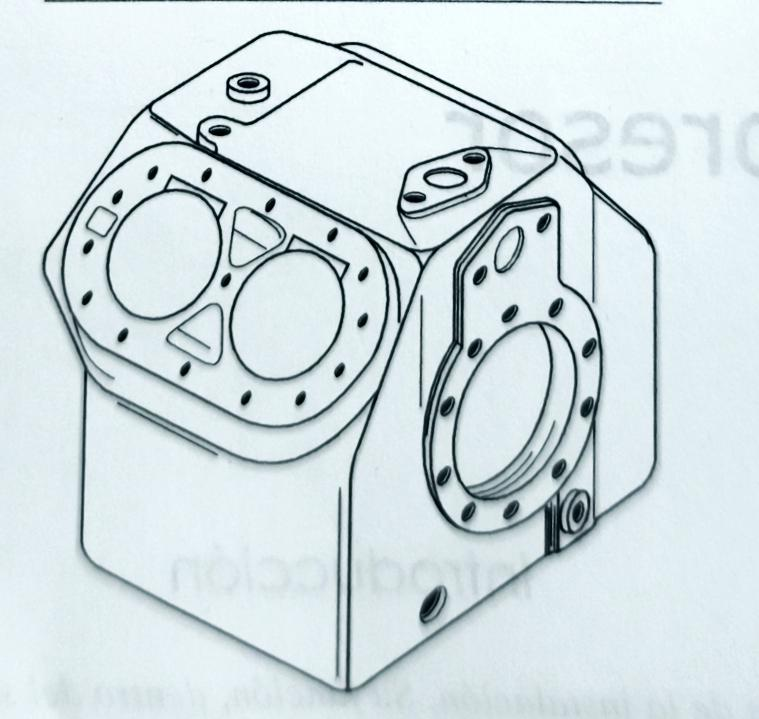
\includegraphics[width=.5\linewidth]{figuras/compresores/bloque}
	\caption{Bloque de un compresor}
	\label{fig:Bloque de un compresor}
\end{figure}

\textbf{C\'arter}

Es el espacio interior comprendido entre el eje cig\"ue\~{n}al y el fondo del bloque, destinado a almacenar el aceite de lubricación.

\textbf{Cilindro}
\begin{wrapfigure}{r}{0.4\linewidth}
	\centering
	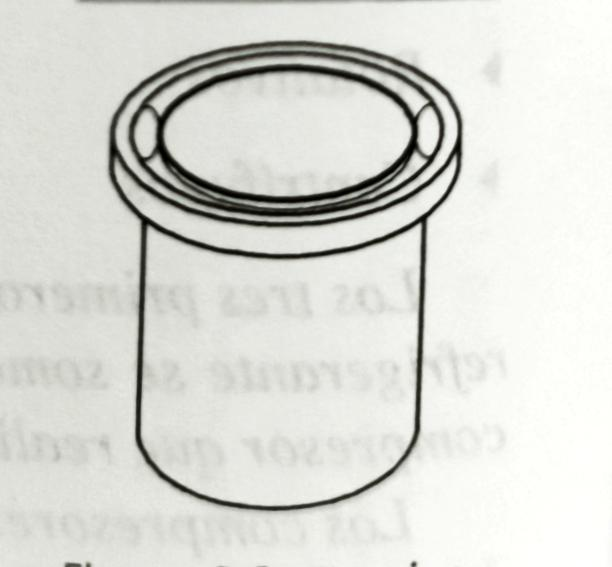
\includegraphics[width=.5\linewidth]{figuras/compresores/cilindro con camisa.jpg}
	\caption{Camisa}
	\label{fig:Camisa}
\end{wrapfigure}
Espacio donde va alojado el pist\'on. En su interior, \'este se desplaza en movimiento rect\'ilineo alternativo. En compresores de mediana y gran potencia (\autoref{fig:Camisa}) lleva camisa, que es una pieza cil\'indrica de acero que lo reviste, y que en casos de desgaste se puede rectificar, o sustituir si procede.

\textbf{Pist\'on o \'embolo}

Elemento que,desplaz\'andose en el interior del cilindro, provoca la aspiraci\'on, compresión y descarga del fluido refrigerante. Lleva alojados los aros o segmentos, que pueden ser:
\begin{itemize}
	\item Aros de engrase: Permiten la lubricación de los cilindros y, en su movimiento, arrastran el aceite al c\'arter.
	\item Aros de compresi\'on: Impiden que el fluido refrigerante escape por los espacios entre el pist\'on y el cilindro, hacia la parte inferior (c\'arter). Esto se aprecia mejor durante la compresi\'on, ya que si hay fugas no se alcanzan las altas presiones necesarias.
\end{itemize}
\textbf{Biela}\\
La biela (\autoref{fig:Conjunto biela-pist\'on y aros}) es el elemento que uno el pist\'on con el eje cig\"ue\~{n}al. Transforma el movimiento circular del eje cig\"ue~{n}al en rectil\'ineo alternativo del pist\'on. Por ello son resistentes y ligeras. La parte superior se llama pie de biela y se une al pist\'on por medio de un bul\'on para evitar el desplazamiento lateral de \'este. Y la parte inferior se llama cabeza de biela y se uno al eje cig\"ue\~{n}al. La biela puede ser de dos tipos, seg\'un se conecte al eje cig\"u\~{n}alo a una exc\'entrica.
\begin{figure}[H]
	\centering
	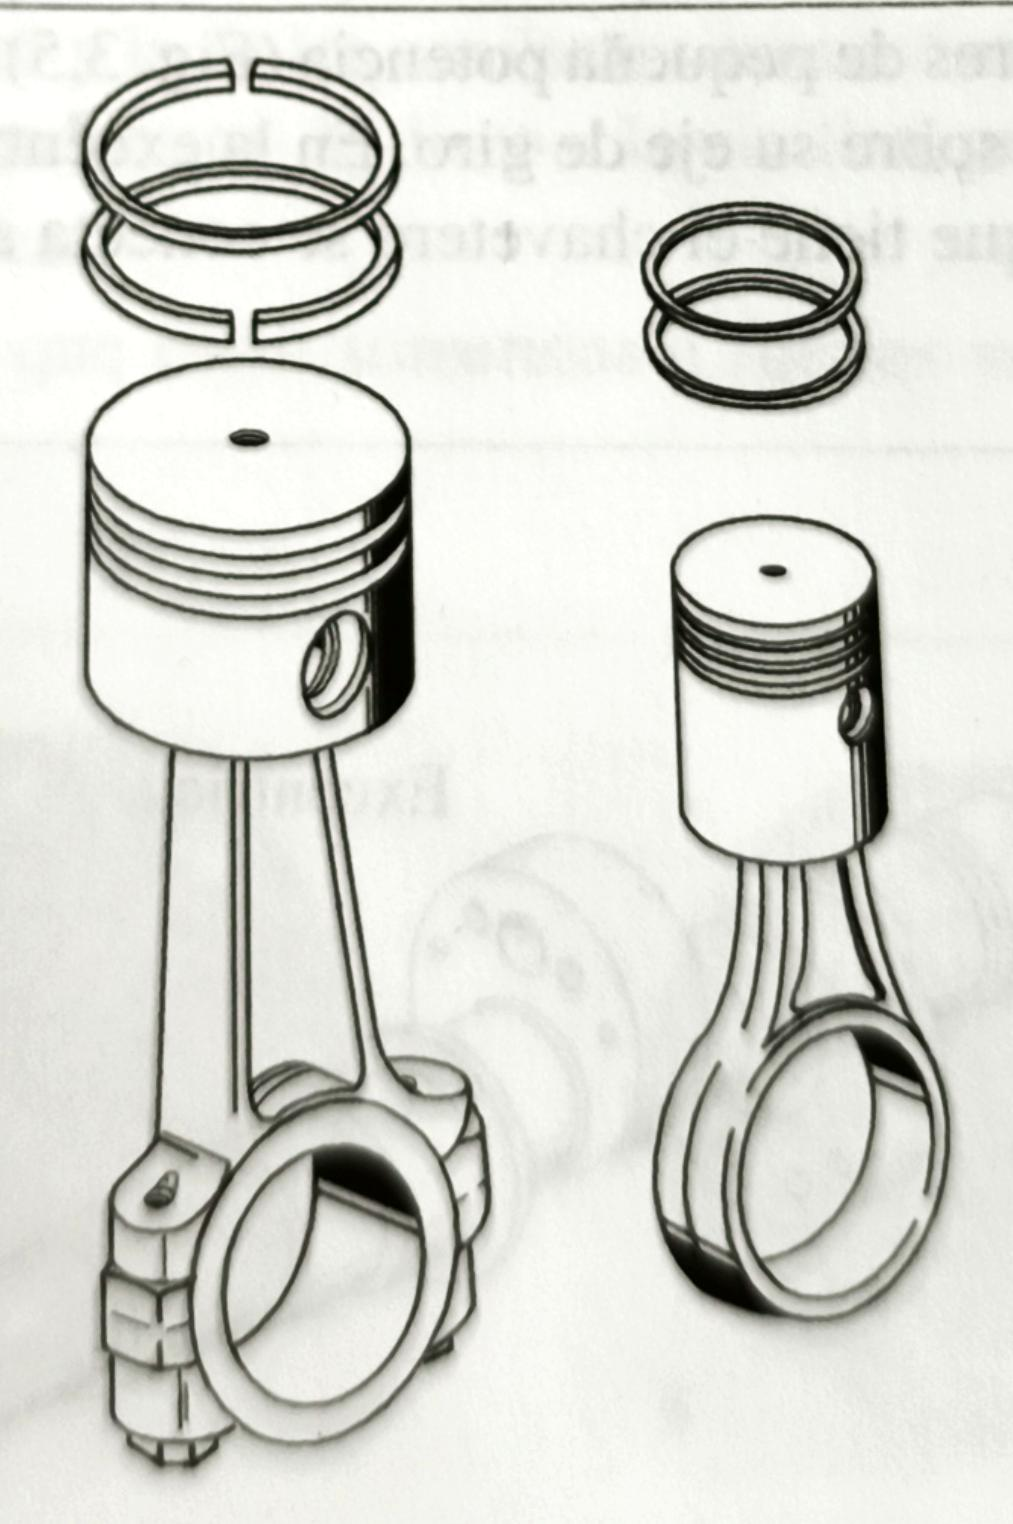
\includegraphics[width=.3\textwidth]{figuras/compresores/piston y biela.jpg}
	\caption{Conjunto biela-pist\'on y aros}
	\label{fig:Conjunto biela-pist\'on y aros}
\end{figure}

\textbf{Eje cig\"ue\~{n}al}\\
La disposici\'on y forma dependen del n\'umero de cilindros (\autoref{fig:Eje cigueñal}). Est\'a formado por un n\'umero determinado de manivelas, que tienen en sus respectivos lados opuestos unos contrapesos de equilibrado. La manivela es la part eque se coencta a la biela.\\
Los extremos del eje, llamados cuellos o mu\~{n}equillas, son los soportes que se apoyan sobe la bancada del compresor. El extremo del eje que tiene el chavetero es el que se conecta al motor el\'ectrico para su accionamiento. El otro extremo acciona la bomba de lubricación.
\begin{figure}[H]
	\centering
	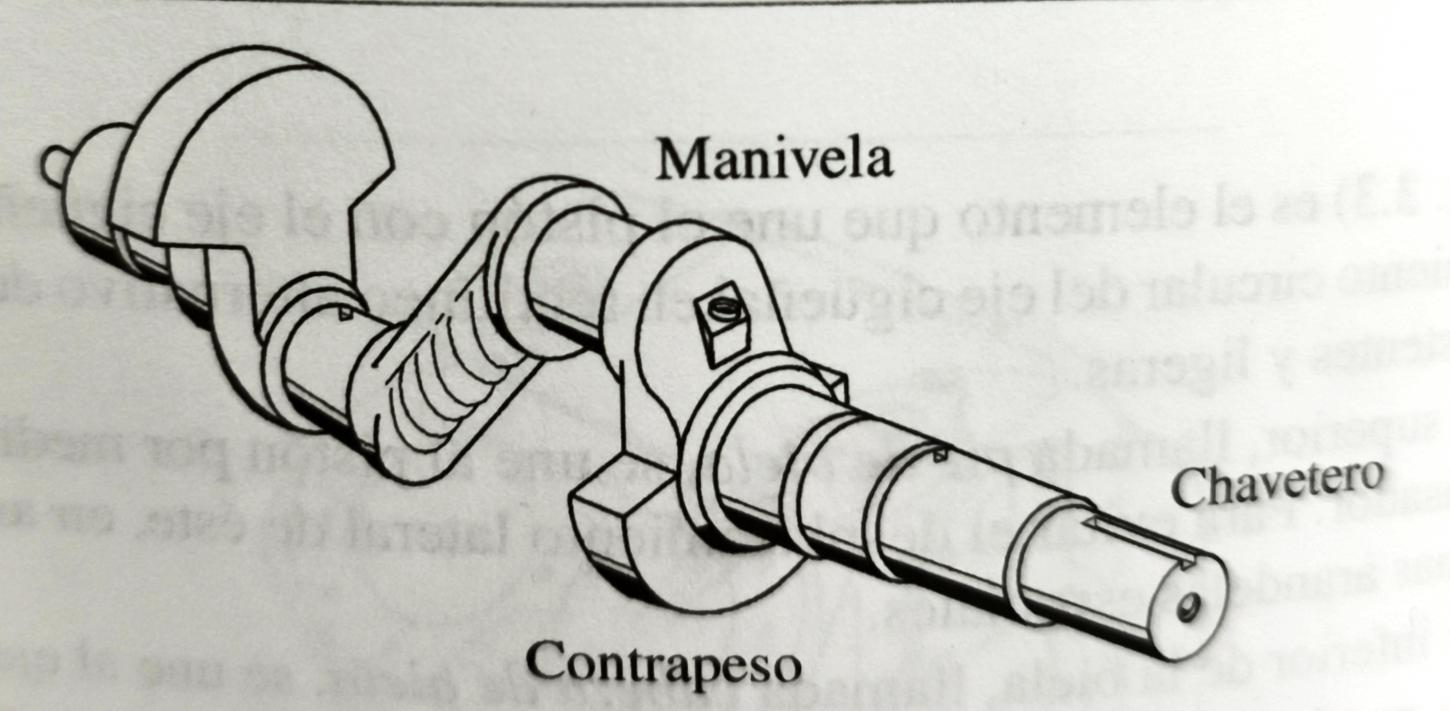
\includegraphics[width=.5\textwidth]{figuras/compresores/eje cigueñal.jpg}
	\caption{Eje cigueñal}
	\label{fig:Eje cigueñal}
\end{figure}
\textbf{Eje de exc\'entrica}\\
Se emplea en compresores de peque\~{n}a potencia (\autoref{fig:Eje de exc\'entrica}). Act\'ua de forma exc\'entrica, de ah\'i el nombre, sobre su eje de giro. En la exc\'entrica se monta la biela. El extremo del eje que tiene el chavetero se conecta al motor el\'ectrico.
\begin{figure}[H]
	\centering
	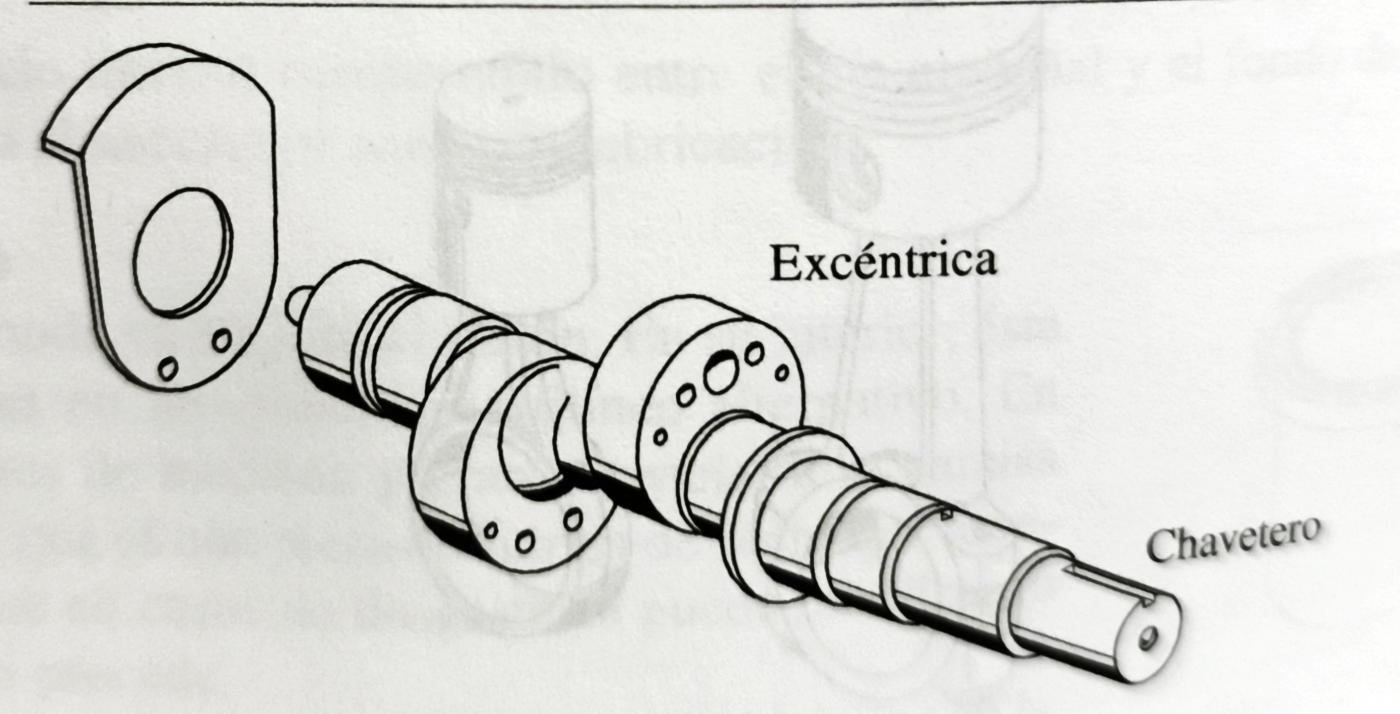
\includegraphics[width=.5\textwidth]{figuras/compresores/eje excentrico.jpg}
	\caption{Eje de exc\'entrica}
	\label{fig:Eje de exc\'entrica}
\end{figure}
\textbf{Culata}\\
Cierra el cilindro por la parte superior. Es la ``tapa'' del cilindro. En ella se alojan las v\'alvulas de aspiración y descarga. Como est\'a sometida a altas temperaturas puede ser refrigerada por aire o por agua (\autoref{fig:Culatas refrigeradas por aire y por agua}).
\begin{figure}[H]
	\centering
	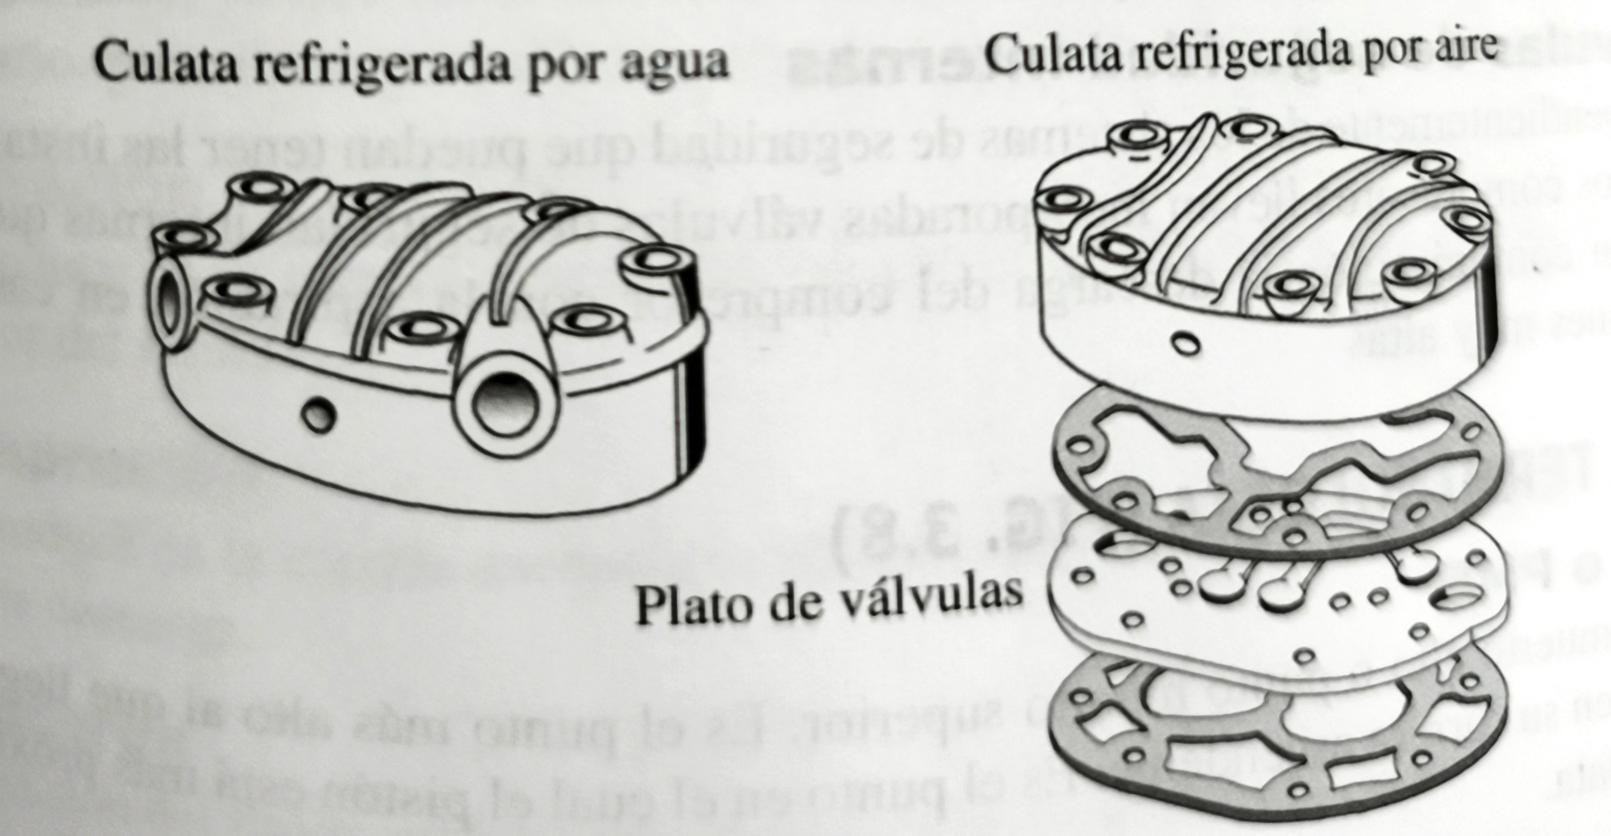
\includegraphics[width=.5\textwidth]{figuras/compresores/culata.jpg}
	\caption{Culatas refrigeradas por aire y por agua}
	\label{fig:Culatas refrigeradas por aire y por agua}
\end{figure}
\textbf{V\'alculas de aspiración y descarga}\\
Se encargan de comunicar el interior del cilindro con los conductos de aspiraci\'on y descarga. Su apertura y cierre se producen por la diferencia de presiones entre la del interior del cilindro y la de los conductos respectivos del fluido. Por lo general son de acero inoxidable, y para grandes potencias, dispotnen de resortes para su accionamiento.\\
\textbf{V\'alvulas de seguridad internas}\\
Independientemente de los sistemas de seguridad que puedan tener las instalaciones, los compresores llevan incorporadas v\'alvulas de seguridad internas que ponen en comunicaci\'on la descargas del compresor con la aspiración en caso de presiones muy altas.

%\subsubsection{Terminología}

%\textbf{PMA o PMS}\\
%Punto muerto alto o punto muerto superio. Es el punto m\'as alto al que llega el pist\'on en su carrera ascendente. Es el punto en el que \'el pist\'on est\'a m\'as cerca de la culata.\\
%\textbf{PMB o PMI}\\
%Punto muerto bajo o punto muerto inferior, es el punto m\'as bajo al que llega el pist\'on en su carrera.\\
%\textbf{Carrera}\\
%Distancia entre el PMS y el PMI. Corresponde a un \'angulo de giro de 180° del cig\"ue\~{n}al.
%
%\begin{figure}[H]
%	\centering
%	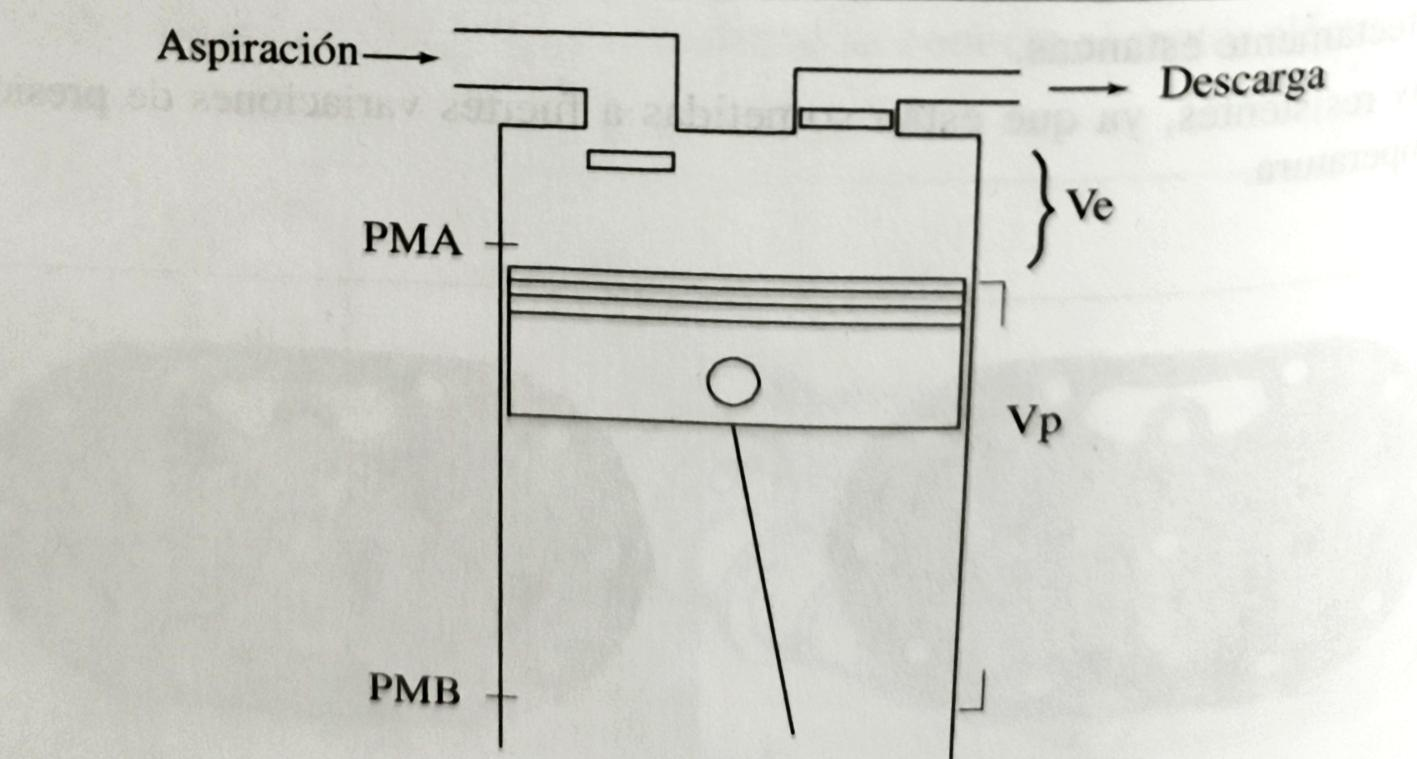
\includegraphics[width=.5\textwidth]{figuras/compresores/terminologia.jpg}
%	\caption{Terminolog\'ia de un cilindro en un compresor}
%	\label{fig:Terminolog\'ia}
%\end{figure}
%
%\textbf{Espacio neutro (Ve)}\\
%Es el comprendido entre el pist\'on cuando se encuentra en el PMS y la culata. Tambi\'en conocido como ``espacio muerto''.Tiene gran importancia en el rendimiento del compresor y est\'a determinado para evitar que el pist\'on, en su carrera ascendente, llegue a chocar con la culata, incluyendo las dilataciones que sufren los materiales, ya que est\'an sometidos a altas temperaturas. Debe ser el m\'inimo necesario, pues tiene gran repercusi\'on en el rendimiento volum\'etrico.\\
%\textbf{Aspiraci\'on}\\
%Se produce en la carrera descendente del pist\'on. Es la admisi\'on del fluido en el interior del cilindro.\\
%\textbf{Compresi\'on}\\
%Se produce en la carrera ascendente del pist\'on e inmediatamente despu\'es se realiza la descarga.\\
%\textbf{Descarga}\\
%Impulsi\'on del fluido refrigerante al conducto de descarga.\\
%\textbf{Volumen desplazado por el pist\'on (Vd)}\\
%El comprendido entre el PMS y PMI que desplaza el pist\'on en la carrera.\\
%\textbf{Volumen total del cilindro (Vt)}\\
%El comprendido entre el pist\'on cuando se encuentra en el PMI y la culata.
%\begin{equation*}
%	Vt = Ve + Vd
%\end{equation*}
%\textbf{Potencia indicada}\\
%Es la potencia que se genera en el interior del cilindro.\\
%\textbf{Potencia efectiva}\\
%Es la potencia que se debe suministrar con el motor el\'ectrico para que el compresor trabaje en las condiciones previstas. Es decir, es la potencia medida en el eje del compresor. Pero a partir de este punto se produce una disminuci\'on de la potencia ya que una parte de la misma se pierde en vencer los rozamientos de cojinetes, bielas, etc. Por ello, la potencia efectiva siempre ser\'a superior a la potencia indicada.
%\begin{equation*}
%	Pe > Pi
%\end{equation*}
%La potencia efectiva es la potencia de accionamiento.\\
%\textbf{Rendimiento mec\'anico}\\
%Es el valor que contempla las p\'erdidas de origen mec\'anico anteriormente mencionadas. Por lo tanto, es la relaci\'on entre ambas potencias:
%\begin{equation*}
%	\eta m = \frac{Pi}{Pe}
%\end{equation*}
\subsubsection{Funcionamiento}
Para facilitar su comprensi\'on vamos a ver como se producen los movimientos de apertura y cierre de las v\'alvulas de aspiraci\'on y descarga, con relaci\'on al movimiento del pist\'on.
\begin{enumerate}[a.]
	\item Carrera descendente:\\ Cuando el pistçón inicia la carrera descendente, hacia el PMI, crea en el interior del cilindro una depresi\'on que implica, que en su interior la presi\'on sea inferior a la existente en la parte superior de la v\'alvula, es decir en el conducto de aspiraci\'on, con lo que la v\'alvula de aspiraci\'on se abre (``baja'') y el fluido refrigerante entra en el cilindro.\\ El fluido entrar\'a en el cilindro hasta que se igualen las dos presiones, y en teor\'ia deber\'ia ser en cantidad igual a la correspondiente al volumen del cilindro, pero hay factores que impiden que entre esa cantidad.\\ La v\'alvula de descarga permanece cerrada, por la alta presi\'on existente en el conducto de descarga mientras el pist\'on se va acercando al PMI y la v\'alvula de aspiraci\'on contin\'ua abierta.\\ As\'i, cuando el pist\'on llega al PMI, la v\'alvula de aspiraci\'on est\'a abierta y la de descarga cerrada. El cig\"ue\~{n}al ha girado 180°.
	\item Carrera ascendente:\\ Cuando el pist\'on rebasa el PMI se inicia la carrera ascendente, y la v\'alvula de aspiraci\'on se cierra, porque la presi\'on en el interior del cilindro es superior a la existente en el conductor de aspiraci\'on. Con las dos v\'alvulas cerradas se inicia la compresi\'on del fluido (\autoref{fig:Carrera ascendente}A), y se produce:
	\begin{itemize}
		\item Una disminici\'on de volumen.
		\item Un aumento de la presi\'on y la temperatura, hasta que la primera alcanza un valor tal que hace que se abra (levante) la v\'alvula de descarga.
	\end{itemize}
	En la \autoref{fig:Carrera ascendente} se puede apreciar que poco antes de que el pist\'on llegue al PMS la v\'alvula de descarga abre (``hacia afuera''), porque la presi\'on en el interior del cilindro, en la carrera escendente, es superior a la del conducto de descarga y ``levanta'' la v\'alvula. El fluido es impulsado hacia el condensador.\\
	El cig\"ue\~{n}al ha girado 180°, con lo que las dos carreras consecutivas gir\'o 360°, es decir una vuelta.\\ Una vez rebasado el PMS, y con la v\'alvula de descarga cerrada, se reinicia el ciclo.
\end{enumerate}
\begin{figure}[H]
	\centering
	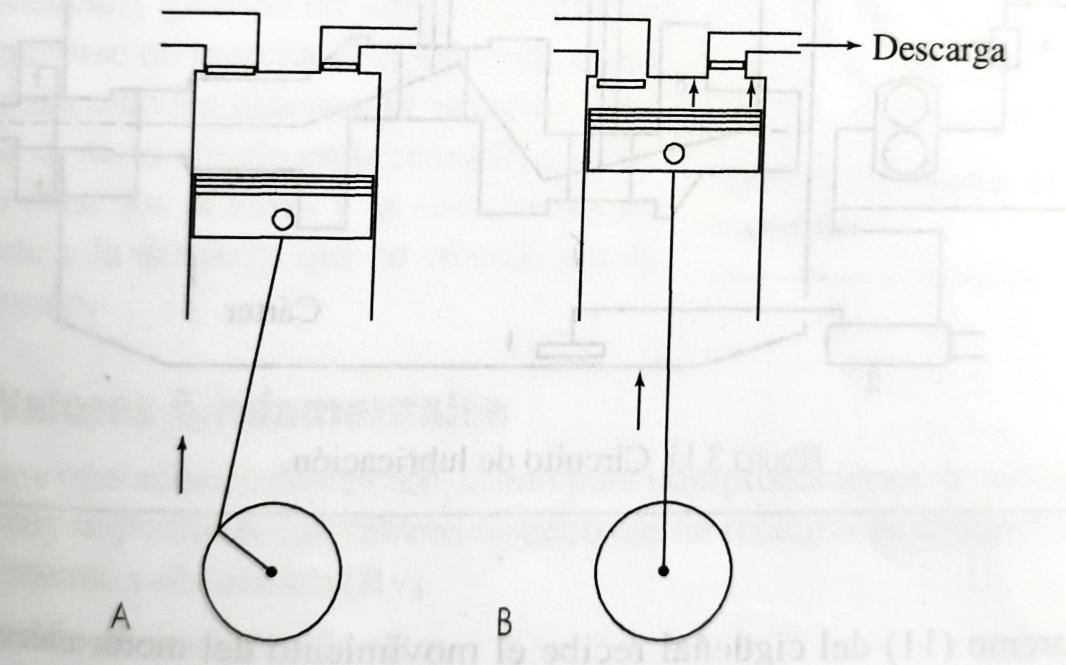
\includegraphics[width=.5\linewidth]{figuras/compresores/aspiracion y descarga.jpg}
	\caption{A = Compresi\'on. B = Descarga}
	\label{fig:Carrera ascendente}
\end{figure}
\subsubsection{Lubricación}
Es uno de los asprectos m\'as importantes del compresor y por lo tanto de la instalaci\'on. El tipo de lubricaci\'on empleada es forzada, mediante una bomba de engranajes que es accionada por el mismo motor el\'ectrico que acciona el compresor.\\ Anteriormente hemos comentado que a trav\'es de los aros de engrase, el aceite sale impulsado hacia las camisas. Pero tambi\'en se lubrican otras partes en movimiento como el cigueñal, cojinetes de bancada, cojinetes de biela y prensas principales.

Es importante saber que el circuito de aceite que conecta la bomba de engranajes con los dispositivos a lubricar cuenta con filtros y un enfriador de aceite, ya que este, adem\'as de lubricar, refrigera los elementos. El compresor tendr\'a enfriador de aceite dependiendo de su potencia, tipo y caracter\'isticas de funcionamiento.
\subsubsection{Valores fundamentales}
Tanto para operaciones de c\'alculo, como para comprobaciones de funcionamiento, son muy importantes los valores respectivos de relaci\'on de compresi\'on (Rc) y de rendimiento volum\'etrico (Rv).
\begin{enumerate}[1.]
	\item \textbf{Relaci\'on de compresi\'on (Rc)}
	\begin{equation*}
		Rc = \dfrac{\text{Presi\'on de descarga absoluta}}{\text{Presi\'on de aspiraci\'on absoluta}}
	\end{equation*}
	$\text{Presi\'on absoluta = Presi\'on manom\'etrica + Presi\'on atmosf\'erica}$
	\item \textbf{Rendimiento volum\'etrico (Rv)}\\ Se puede expresar de varias maneras, pero una de ellas a efectos pr\'acticos es:
	\begin{equation*}
		Rv = {\frac{\text{Volumen de vapor que realmente aspira}}{\text{Volumen te\'orico que tendr\'ia que aspirar}}X 100}
	\end{equation*}
	Cuanto mayor sea la relaci\'on de compresi\'on, menor ser\'a el rendimiento volum\'etrico y viceversa.

	Su valor depende de factores rales como el espacio neutro y la densidad del fluido en el interior del cilindro.
	\item \textbf{Volumen desplazado}\\ El volumen de fluido que en teor\'ia tiene que aspirar es el volumen desplazado por el pist\'on en su carrera. Como sabemos, el volumen de un cilindro es el producto del \'area por la altura:
	\begin{gather*}
		V = S \times h\\ 
		S = \pi\cdot r^2 = \pi\cdot(\frac{D}{2})^2 = \pi\cdot\frac{D^2}{4}
	\end{gather*}
	y la altura (h) es la distancia entre PMI y el PMS, o sea es la carrera:
	\begin{equation*}
		V = \frac{\pi D^2}{4}C
	\end{equation*}
	que es el volumen que desplaza el pist\'on en una revoluci\'on. Si gira el cig\"ue\~{n}al a n revoluciones por minuto y tiene N cilindros, el volumen desplazado ser\'a:
	\begin{equation*}
		Vd = \frac{\pi\cdot D^2\cdot C\cdot n\cdot N\cdot 60\cdot 10^-3}{4}(\frac{m^3}{h})
	\end{equation*}
\end{enumerate}
\subsection{Compresores herméticos}
Su \'ambito de aplicaci\'on comprende los sitemas de refrigeraci\'on y aire acondicionado.\\El motor el\'ectrico va acoplado directamente al compresor, y ambos dentro de la misma envolvente (carcasa) de acero formando una unidad. Al ser herm\'eticos (cerrados) no podemos acceder a ellos, como por ejemplo, para realizar operaciones de mantenimiento. Pueden ser alternativos, rotativos o de tornillo.\\ En su configuraci\'on (\autoref{fig:Compresor herm\'etico}), lleva tres tubos soldados a la carcasa. Dos son del mismo di\'ametro y el tercero menor. El de menor di\'ametro se conectar\'a a la descarga y la aspiraci\'on a cualquiera de los otros dos. Por lo general, se hace al tubo que est\'a al lado contrario de la placa de conexionado el\'ectrico, para evitr que las condensaciones que se puedan producir en el exterior del mismo, lleguen a introducirse a la placa.\\ De esta manera el otro tubo, que no se conecta la circuito, se puede utilizar para que, despu\'es de instalar una conexi\'on ob\'us o una v\'alvula de intervenci\'on, se aproveche para realizar operaciones tales como:
\begin{itemize}
	\item Meter carga de refrigerante
	\item Comprobar la presi\'on de aspiraci\'on
	\item Comprobar la temperatura de evaporaci\'on
	\item Meter aceite
\end{itemize}
\begin{figure}[H]
	\centering
	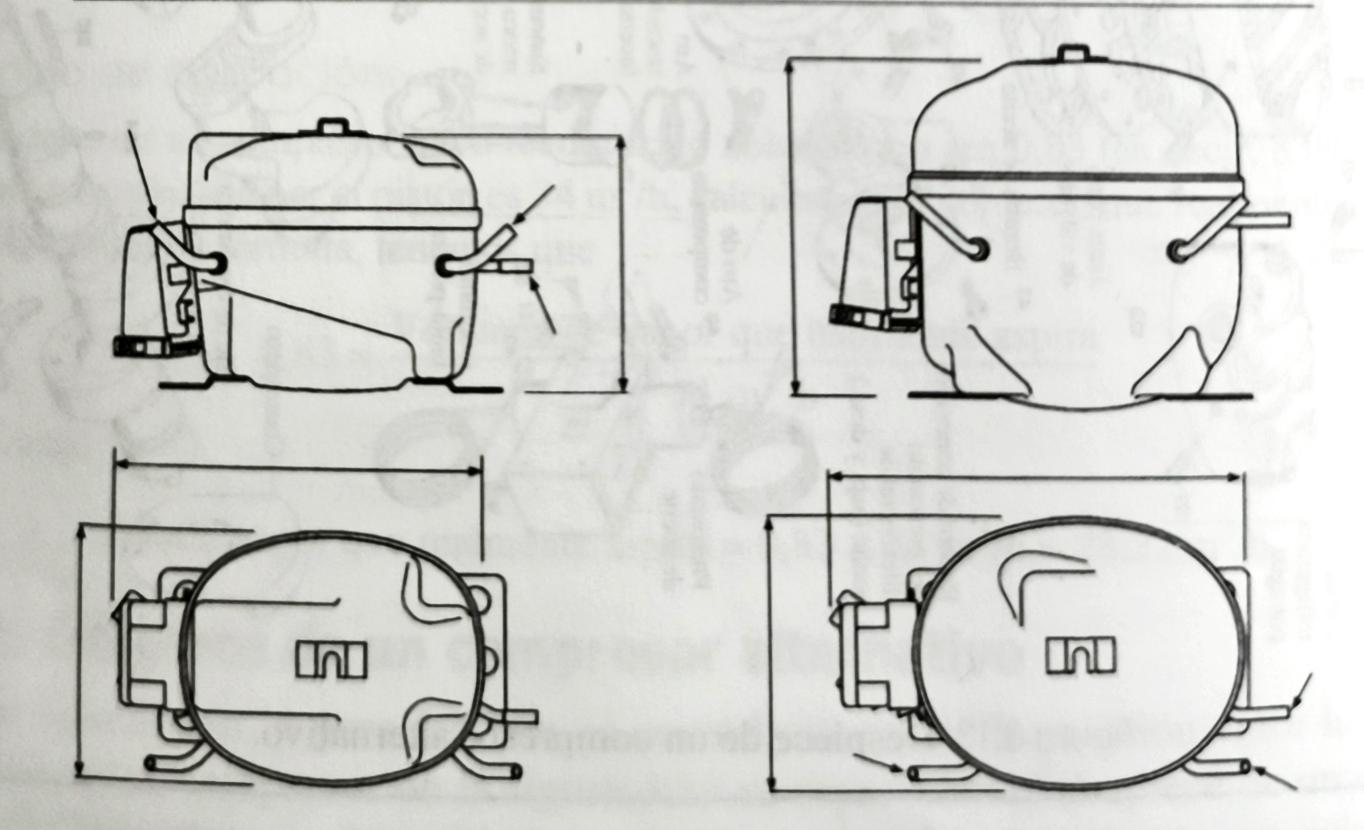
\includegraphics[width=.8\linewidth]{figuras/compresores/compresor herméticos.jpg}
	\caption{Compresor herm\'etico}
	\label{fig:Compresor herm\'etico}
\end{figure}
\subsubsection{Algunas caracter\'isticas}
\begin{enumerate}[1.]
	\item Son silenciosos porque cuentan con resortes interiores y c\'amaras silenciadoras que amortiguan el golpeteo de las v\'alvulas. Carecen de transmisiones exteriores como por ejemplo correas.
	\item Est\'an refrigeradores por el fluido de aspiraci\'on por lo que, la falta de fluido afectar\'ia a la refrigeraci\'on del compresor. Hay que evitar la humedad en el circuito y la entrada de l\'iquido al compresor porque estar\'ian en contacto con la parte el\'ectrica.
	\item Trabajar a temperaturas inferiores a las normales, implicar\'ia el aumento del volumen espec\'ifico, que afectar\'ia, entre otras cosas a la refrigeraci\'on.
\end{enumerate}
\subsection{Compresores semiherméticos}
Estos compresores en su funcionamiento tienen las mismas ventajas e inconvenientes que los herm\'eticos pero a diferencia que son m\'as accesibles para realizar mantenimiento. Por ejemplo, en compresores semiherm\'eticos alternativos se pueden desmontar para realizar operaciones de mantenimiento tales como cambiar pistones o aros.\\ Pueden ser enfriados externamente por aire o por agua.
\subsubsection{\'Acidos}
Es importante comentar que en los compresores, ya sean herm\'eticos o semiherm\'eticos, una de las aver\'ias m\'as importantes es la contaminaci\'on del circuito por \'acidos, puesto que se refrigeran por los vapores de aspiraci\'on. La presencia de \'acidos se produce por altas temperaturas en la zona que se encuentra entre el estator y rotor, esto genera que el fluido refrigerante reaccione y ataque los devanados del estator.\\ Las causas pueden ser varias pero se podr\'ia englobar en mantenimiento inadecuado, sobre carga del motor y elevadas temperaturas de trabajo.\\ Si se cambia un compresor por otro en un sistema contaminado por \'acidos y antes no se eliminan \'estos, atacar\'an a los aislamientos de los bobinados, con lo cual la duraci\'on del nuevo compresor ser\'a muy corta.
\subsection{Compresores abiertos}
Se llaman abiertos porque el motor el\'ectrico y el compresor est\'an separados. Por lo tanto, el fluido refrigerante ya no est\'a en contacto con la parte el\'ectrica, como ocurre en los compresores herm\'eticos y semiherm\'eticos. Como est\'an separados la conexi\'on entre ambos necesita de un sistema de estanqueidad o sello en ese punto para evitar las fugas del fluido refrigerante al exterior. El acoplamiento motor-compresor se puede realizar mediante correas, se puede adaptar la velocidad con sus di\'ametros (seg\'un necesidad de carga) o mediante dos platos met\'alicos unidos el\'asticamente.
\subsubsection{Caracter\'isticas de funcionamiento}
En estos compresores abiertos se considera buena relaci\'on de compresi\'on (Rc) si no excede de 10:1, ya que cuanto menor sea, mayor ser\'a el rendimiento volum\'etrico (Rv) y, por lo tanto, mayor ser\'a la potencia frogir\'ifica.\\ Si el compresor tuviera que trabajar con una Rc elevada, como sucede, por ejemplo, cuando se trata de instalaciones que necesiten temperaturas muy bajas para enfriar y las de condensaci\'on sean normales, entonces no se podr\'ia utilizar uno de simple etapa, porque entre otras cosas, las altas temperaturas afectar\'ian:
\begin{itemize}
	\item A los materiales (dilataciones)
	\item A la lubricaci\'on, perjudicar\'ia la viscosidad del aceite
	\item A las temperaturas de descarga, porque ser\'ian muy altas
	\item Y a los rendientos, que disminuir\'ian
\end{itemize}
Para solucionar estos inconvenientes tendr\'iamos que recurrir a los compresores de doble etapa (sistema compound), que tambi\'en se hace extensivo a los semiherm\'eticos.
\subsubsection{Compresores de doble etapa}
Los compresores de doble etapa reparten la elevada relaci\'on de presiones y disminuyen el alto recalentamiento. Cada secci\'on del compresor trabaja a menor presi\'on y tambi\'en menor temperatura de descarga, lo que implica un mejor aprovechamiento volum\'etrico. Para ello emplean un sistema de enfriamiento en la etapa intermedia, cuando es asi se los llama sistema por \textbf{inyecci\'on parcial}. Pero cuando se enfria el fluido en la etapa intermedia y, a su vez, antes de que \'este entre en el evaporador se lo llama sistema de \textbf{inyecci\'on total}.
\begin{itemize}
	\item \textbf{Inyecci\'on parcial:}\\ Se mezclan el fluido expansionado por la v\'alvula y los gases de descarga de los cilindros de baja en la tuber\'ia de presi\'on intermedia. De esta manera, se logra bajar la temperatura de descarga de los cilindros de alta.
	\item \textbf{Inyecci\'on total}\\ Se realiza un enfriamiento de los gases de descarga de los cilindros de baja y, a su vez, tambi\'en se hacen pasar el fluido expansionado por un intercambiador de calor para enfriar el refrigerante antes de entrar al evaporador e incrementar el efecto frigorífico.
\end{itemize} 
\subsection{Compresores rotativos}
Se caracterizan por comprimir el fluido refrigerante mediante el movimiento circular continuo de un rotor, que puede ser de exc\'entrica o de paletas.
\subsubsection{De exc\'entrica}
\begin{wrapfigure}{r}{0.45\linewidth}
	\centering
	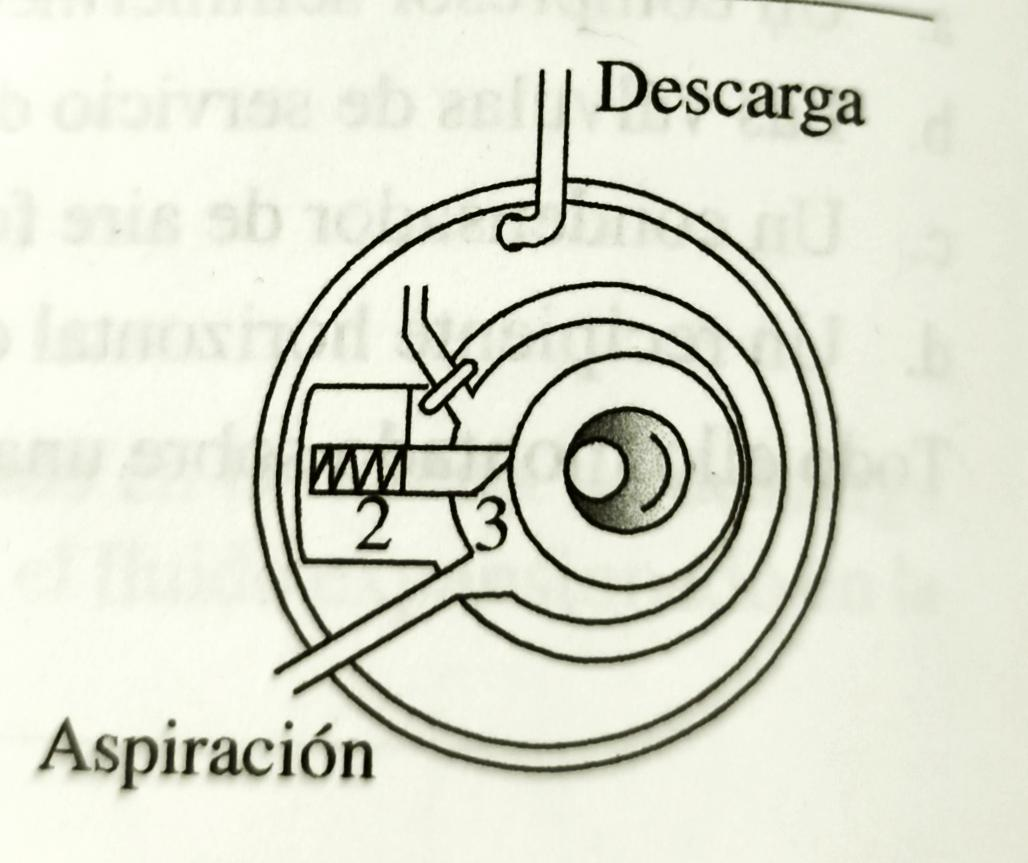
\includegraphics[width=.7\linewidth]{figuras/compresores/rotor de excentrica.jpg}
	\caption{Rotor de exc\'entrica}
	\label{fig:Rotor de exc\'entrica}
\end{wrapfigure}
Consta (\autoref{fig:Rotor de exc\'entrica}) de un rotor exc\'entrico respecto al cilindro donde se aloja y que en su movimiento llega a establecer contacto con \'el.\\Este rotor, por acci\'on del resorte (2) est\'a permanentemente en contacto con una paleta (3).\\Esta paleta, tal como se aprecia en la figura, establece la separaci\'on entre las c\'amaras de aspiraci\'on y de descarga. En su funcionamiento, la aspiraci\'on se realiza de manera continua, y al disminuir el espacio comprendido entre el rotor y el cilindro, se efect\'ua la comprensi\'on del fluido refrigerante y posterior descarga.

\subsubsection{De paletas}

B\'asicamente (\autoref{fig:Rotor de paletas}) consta de un rotor montado en el interior de un cilindro y cuyos centros ent\'an ligeramente desplazados. Este rotor aloja unas paletas que est\'an comprimidas contra la pared del cilindro por medio de unos resortes. Al pasar cada paleta por el orificio de la aspiraci\'on, se crea una depresi\'on que provoca la entrada del fluido en el espacio comprendido entre esa paleta y la anterior. Posteriormete y dado que el espacio entre el rotor y el cilindro disminuye, tambi\'en lo hace el volumen del fluido (compresi\'on) hasta que alcanza el orificio de descarga.\\ Existen compresores cuyos rotores no llevan resortes y las paletas se mantienen comprimidas por la acci\'on de su propio peso y de la fuerza centr\'ifuga.

\begin{figure}[H]
	\centering
	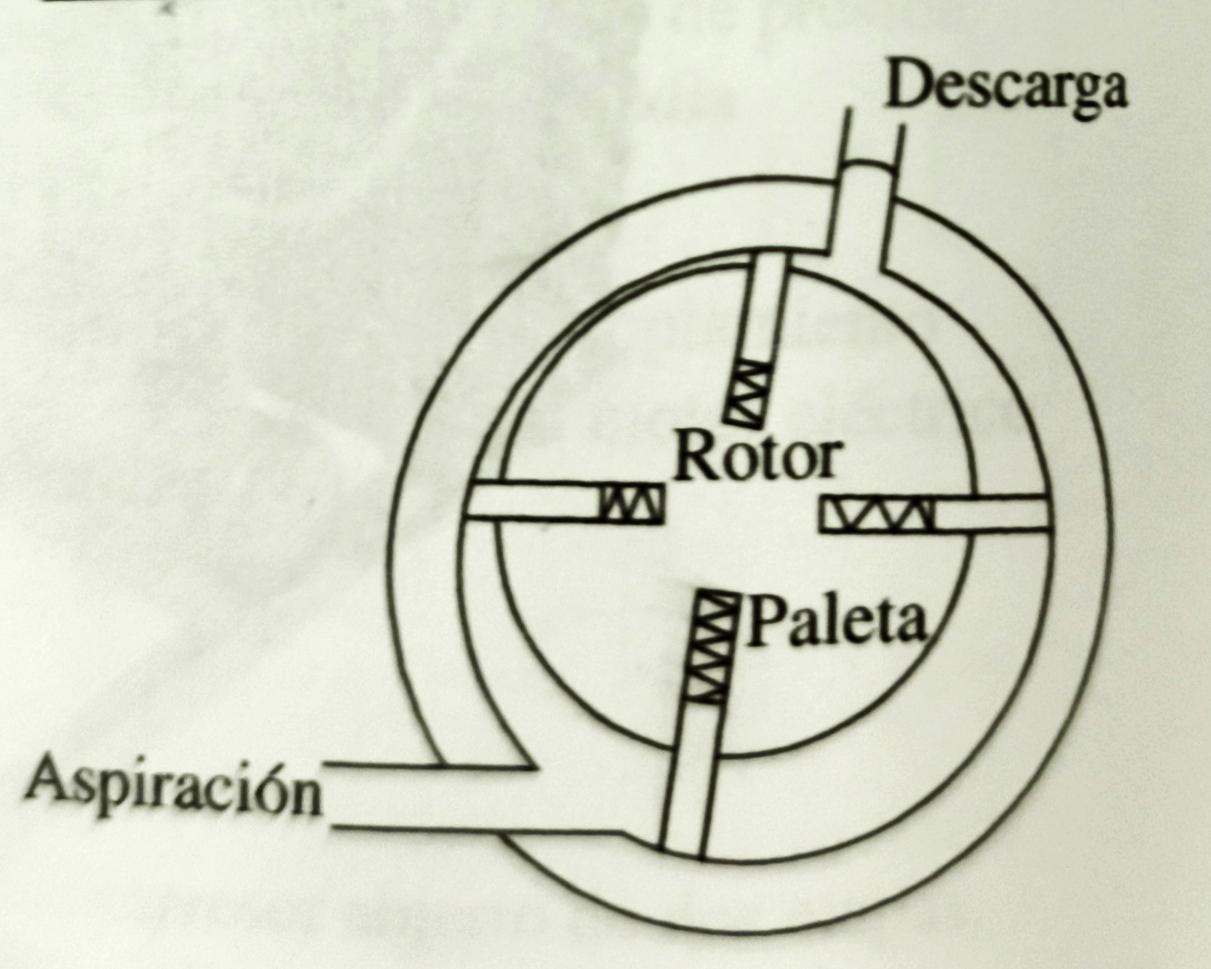
\includegraphics[width=.4\linewidth]{figuras/compresores/rotor de paletas.jpg}
	\caption{Rotor de paletas}
	\label{fig:Rotor de paletas}
\end{figure}

\subsection{Compresores helicoidales}

Los compresores helicoidales o de tornillo son distintos a los anteriormente vistos. La compresi\'on del fluido es continua. Constan de dos rotores llamados primario y secundario que, montados en ambos extremos sobre cojinetes, aseguran su exacta posici\'on en el interior del compresor. El \textbf{rotor primario}, de cuatro l\'obulos o helicoides, es accionado directamente por el motor el\'ectrico y gira a la misma velocidad que \'este.\\ Mediante un sistema de rodamientos, el rotor primario transmite el movimiento al \textbf{rotor secundario}, que tiene seis l\'obulos o helicoides y es del mismo di\'ametro, pero gira a menor velocidad y en sentido contrario.\\ Entre los dos rotores existe una separaci\'on muy pequeña, es decir, no est\'an en contacto entre s\'i.\\Al girar ambos rotores dentro de la cavidad del compresor y debido a esa pequeña separaci\'on, se producen las aberturas de espacios en la zona de aspiraci\'on que con el giro van disminuyendo, con lo que se translada y comprime el fluido hacia el otro extremo de los rotores, donde se produce la descarga del fluido refrigerante.\\ Los hay de tipo herm\'etico, semiherm\'etico y abiertos.
\subsubsection{Importancia del aceite}
Estos compresores helicoidales llevan unos grandes separadores de aceite. Este es inyectado a lo largo de los tornillos para su lubricaci\'on y sellado al mismo tiempo, lo que facilita la compresi\'on del fluido.\\ La \autoref{fig:Circuito de aceite en instalaciones con compresores a tornillo} representa una aplicaci\'on muy utilizada de estos compresores.\\Como consecuencia de la alta temperatura que alcanza el aceite, a la salida del separador y antes de volver al compresor, suele pasar por un enfriador, que seg\'un las caracter\'isticas de la instalaci\'on, puede utilizar aire, agua o el mismo refrigerante para el enfriamiento del aceite.\\ Los factores que determinan si es necesario el enfriamiento del aceite son las condiciones de trabajo:

\begin{itemize}
	\item Temperatura de condensaci\'on
	\item Temperatura de evaporaci\'on
	\item Temperatura de descarga
\end{itemize}

\begin{figure}[H]
	\centering
	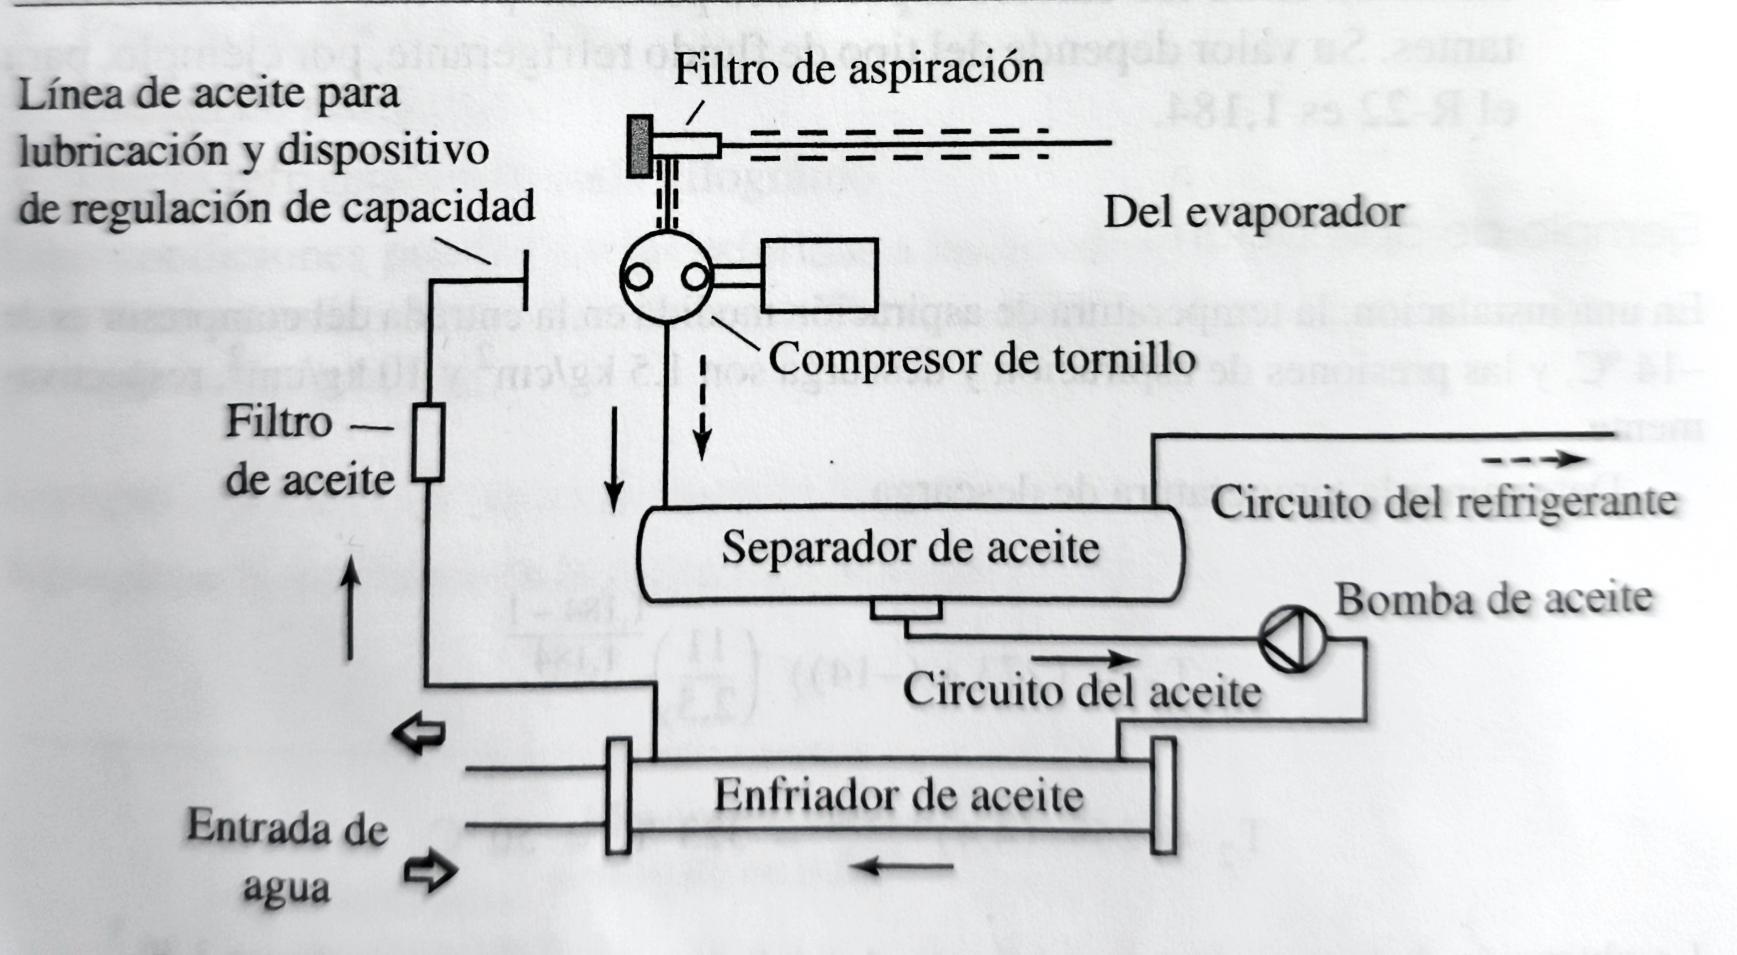
\includegraphics[width=\textwidth]{figuras/compresores/circuito de aceite (2).jpg}
	\caption{Circuito de aceite en instalaciones con compresor a tornillo}
	\label{fig:Circuito de aceite en instalaciones con compresores a tornillo}
\end{figure}

\subsection{Regulación de la potencia}

Si la carga de los evaporadoes siempre fuese la misma, se intalar\'ia el compresor a esa determinada carga t\'ermica. Pero como en la mayor\'ia de los casos la carga var\'ia (ejemplo m\'as notorio lo tenemos en las instalaciones de aire acondicionado), se debe encontrar un punto de equilibrio entre la carga producida por el compresor y la carga necesaria en el evaporador.\\Para los casos de pequeñas instalaciones, como pueden ser heladeras dom\'esticas, el compresor consume muy poca potencia. Por tanto estas instalciones generalmente trabajan con un sistema ON-OFF, donde consumen la potencia m\'axima y una vez que se llego al set point se apaga el compresor.\\En cambop en instalaciones de mayores potencias hay que conseguir un equilibrio entre la carga producida y la necesaria, lo cual significa menores consumos y menos mantenimiento.

\subsubsection{Sistema de regulaci\'on}

La regulaci\'on se puede realizar de varias maneras, por ejemplo actuando sobre el volumen desplazado o bien sobre las revoluciones del motor, ya que la potencia es directamente proporcional a las revoluciones.\\Acontinuaci\'on se presenta un sistema de regulaci\'on para compresores a tornillo:

\begin{enumerate}[a.]
	\item Instalando entre la parte inferior de los rotores y el fondo del c\'arter un dispositivo deslizante (pist\'on), que es accionado por la presi\'on del aceite (mediante electrov\'alvula), y que al desplazarse a lo largo de los rotores, su posici\'on marca el ``punto'' de inicio de la compresi\'on del fluido y determina as\'i el desplazamiento volum\'etrico del compresor.
	\item Mediante controles deslizantes (pistones) instalados en el extremo final de la brida de descarga.
\end{enumerate}

La \autoref{fig:Disposici\'on de los controles de capacidad} representa un compresor semiherm\'etico, en vista superior. La entrada de fluido refrigerante es a trav\'es de la v\'alvula de aspiraci\'on situada en el lado izquierdo, y la descarga (oculta) est\'a en el lado derecho.\\La regulaci\'on de la potencia se realiza mediante las dos electrov\'alvulas y los dos pistones montados en el extremos de la brida de descarga (m\'etodo b.)

\begin{figure}[H]
	\centering
	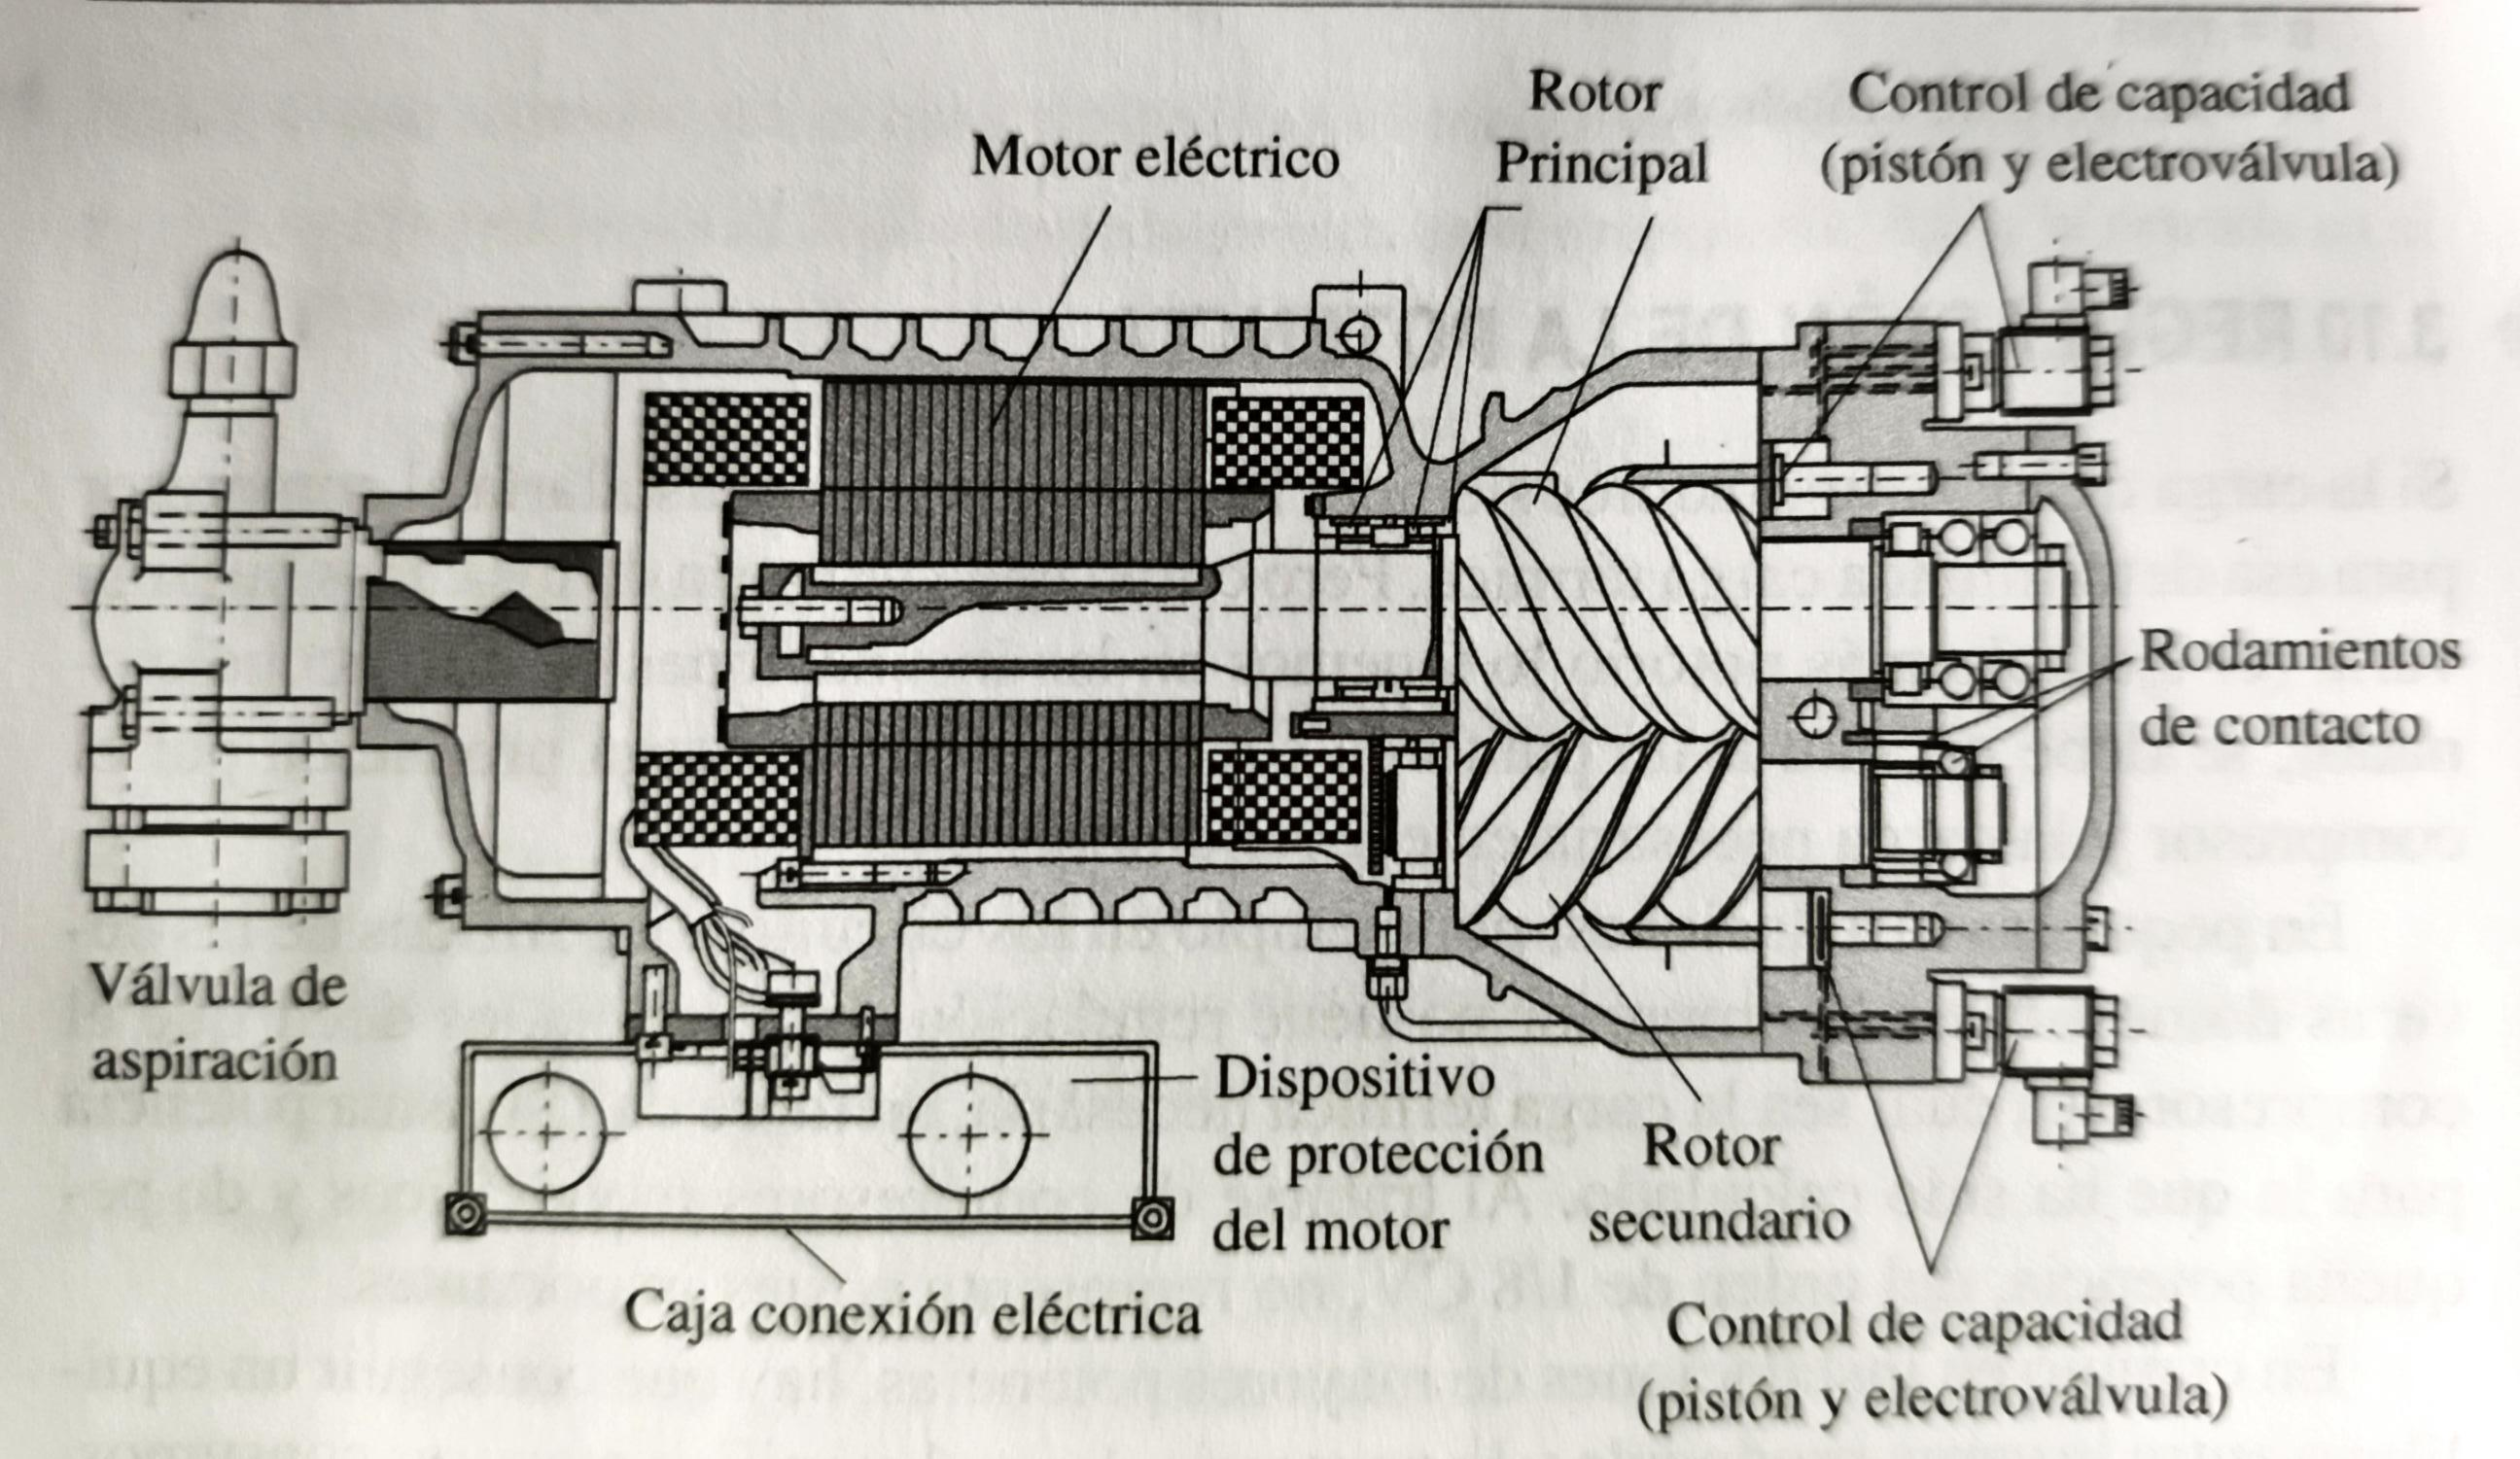
\includegraphics[width=\textwidth]{figuras/compresores/controles de capacidad.jpg}
	\caption{Disposici\'on de los controles de capacidad}
	\label{fig:Disposici\'on de los controles de capacidad}
\end{figure}

\begin{wrapfigure}{r}{0.5\linewidth}
	\centering
	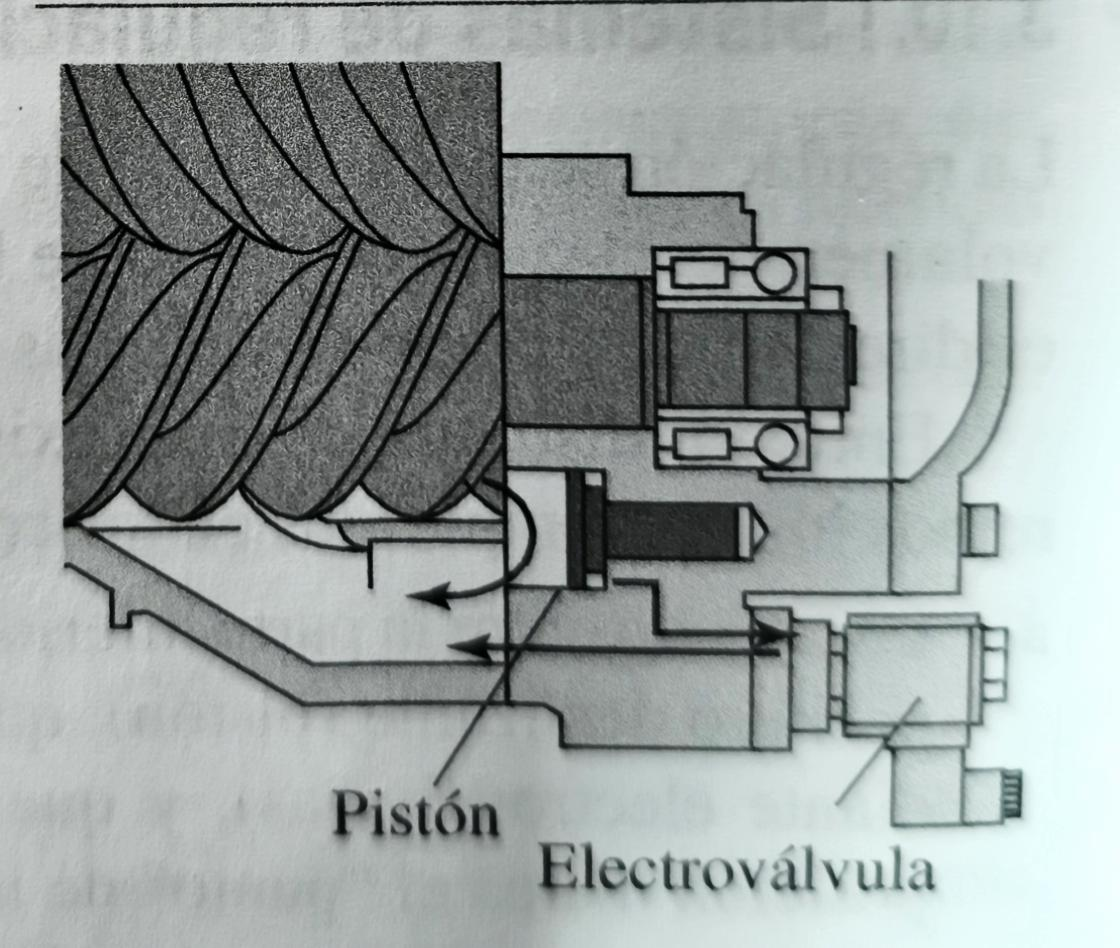
\includegraphics[width=.7\linewidth]{figuras/compresores/detalle de control de capacidad.jpg}
	\caption{Detalle de control de capacidad}
	\label{fig:Detalle de control de capacidad}
\end{wrapfigure}

Los dos pistones son accionados hidr\'aulicamente. Mediante una señal el\'ectrica se abren unos orificios debidamente calibrados, y as\'i una parte del fluido es conducido hacia el lado de la aspiraci\'on (en la \autoref{fig:Detalle de control de capacidad} se aprecia en detalle la operaci\'on)\\Al disminuir el caudal de fluido descargado, tambi\'en se disminuye la potencia. En este sistema, la regulaci\'on de potencia se realiza en dos etapas. Cuando una electrov\'alvula no \'esta activada, se produce una reducci\'on de potencia.

\subsection{Variaciones de las presiones y su repercursión en las potencias}

La potencia frigor\'ifica de un compresor dependen de las condiciones de trabajo. Por ello vamos a ver de que manera repercuten en la potencia frigor\'ifica las variaciones de las presiones de trabajo.\\ En el diagrama de Mollier podemos apreciar c\'omo var\'ia la potencia frigor\'ifica seg\'un las distintas temperaturas de evaporaci\'on y condensaci\'on.
% \renewcommand{\theenumi}{\alph{enumi}}
\begin{enumerate}[a.]
	\item ¿Qu\'e ocurre cuando la presi\'on de aspiraci\'on disminuye?\\ Supongamos que la presi\'on de aspiraci\'on $Pa$, disminuye hasta un valor $Pa^\prime$\\Se comprueba que:
	\begin{enumerate}[1.]
		\item Al disminuir la presi\'on de aspiraci\'on, el efecto refrigerante ($ER^\prime$) tambi\'en disminuye con lo cual disminuye la potencia.
		\item El volumen espec\'ifico ($Ve^\prime$) aumenta, lo que implica que el desplazamiento volum\'etrico disminuye.
	\end{enumerate}

	\begin{figure}[H]
		\centering
		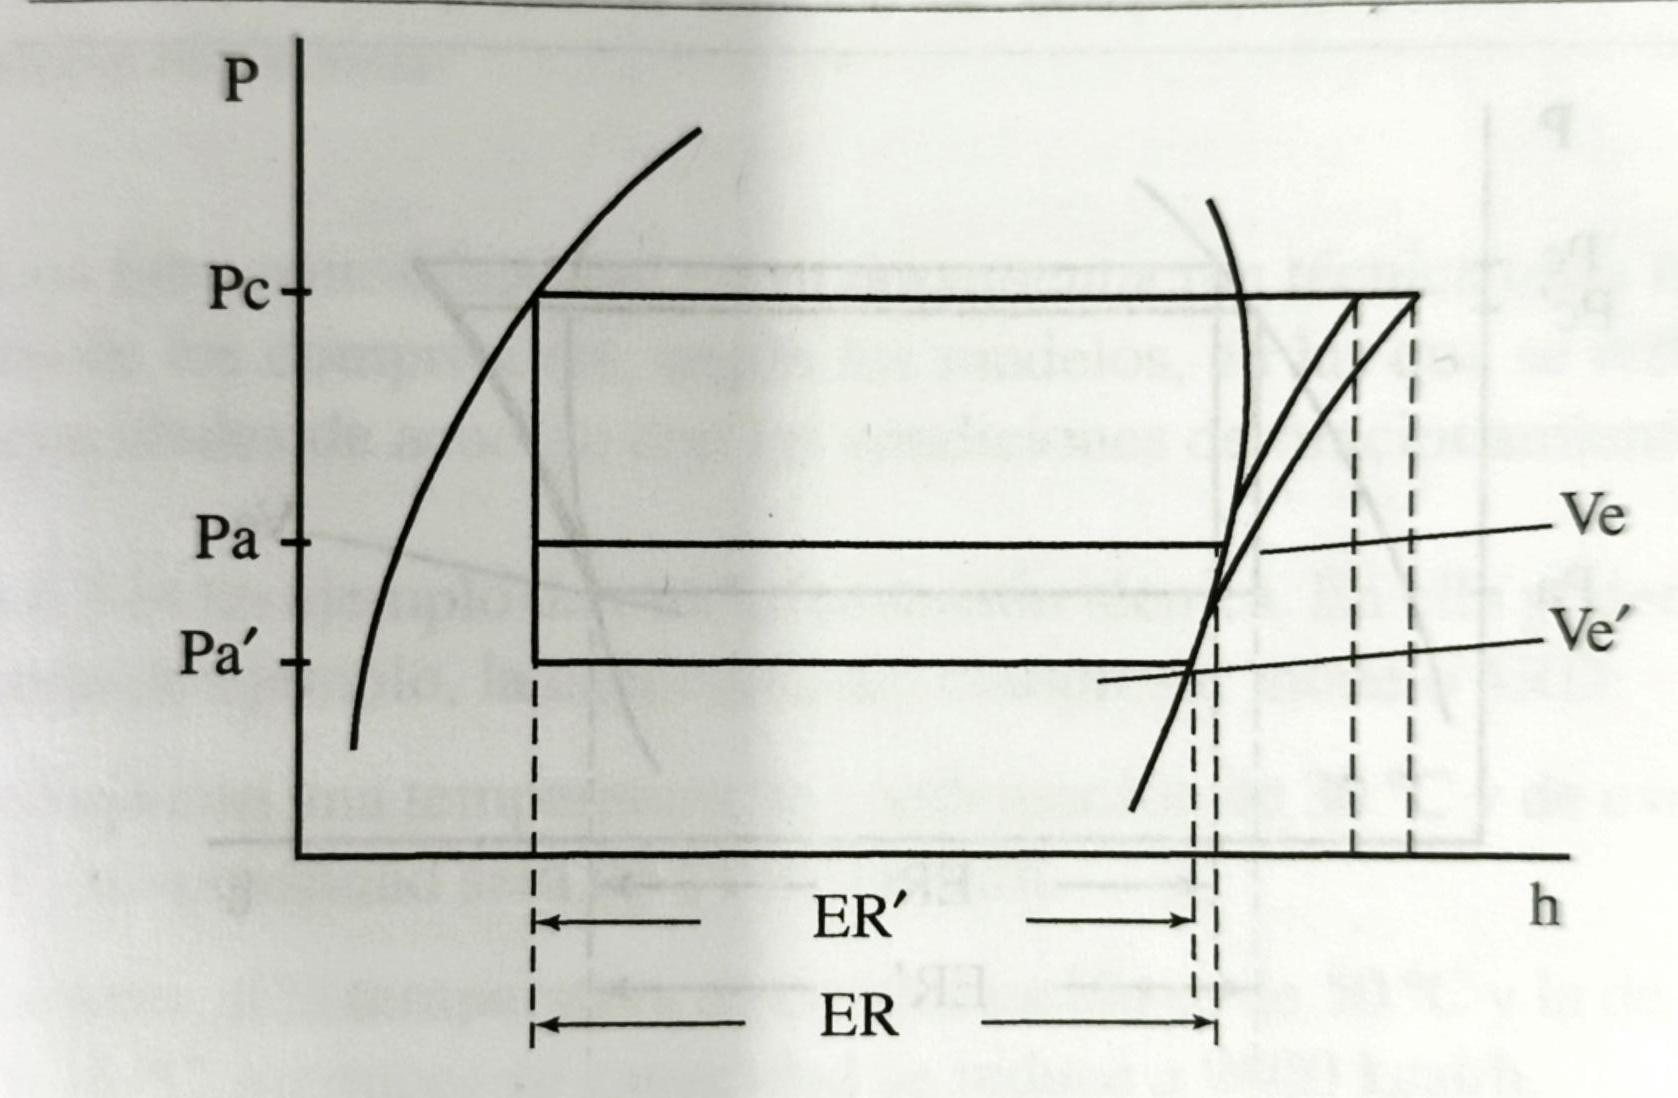
\includegraphics[width=.6\textwidth]{figuras/compresores/variacion de la presion de aspiracion.jpg}
		\caption{Variaci\'on de la psei\'on de aspiraci\'on en el diagrama p-h.}
		\label{Variaci\'on de la presi\'on de aspiraci\'on}
	\end{figure}
	Tambi\'en se puede demostrar num\'ericamente con la relaci\'on de compresi\'on (Rc) para este caso aumenta, por tanto disminuye el rendimiento volum\'etrico (Rv) y la potencia frigor\'ifica.

	\item ¿Qu\'e ocurre con la potencia frigor\'ifica cuando disminuye la presi\'on de condensaci\'on?\\Viendo la \autoref{fig:Variaci\'on de la presi\'on de condensaci\'on} se puede ver que:
	\begin{enumerate}[1.]
		\item El efecto refrigerante ($ER^\prime$) aumenta, con lo que la potencia frigor\'ifica tambi\'en aumenta.
		\item La relaci\'on de compresi\'on (Rc) disminuye, con lo que la potencia frigor\'ifica aumenta.
	\end{enumerate}
	\begin{figure}[H]
		\centering
		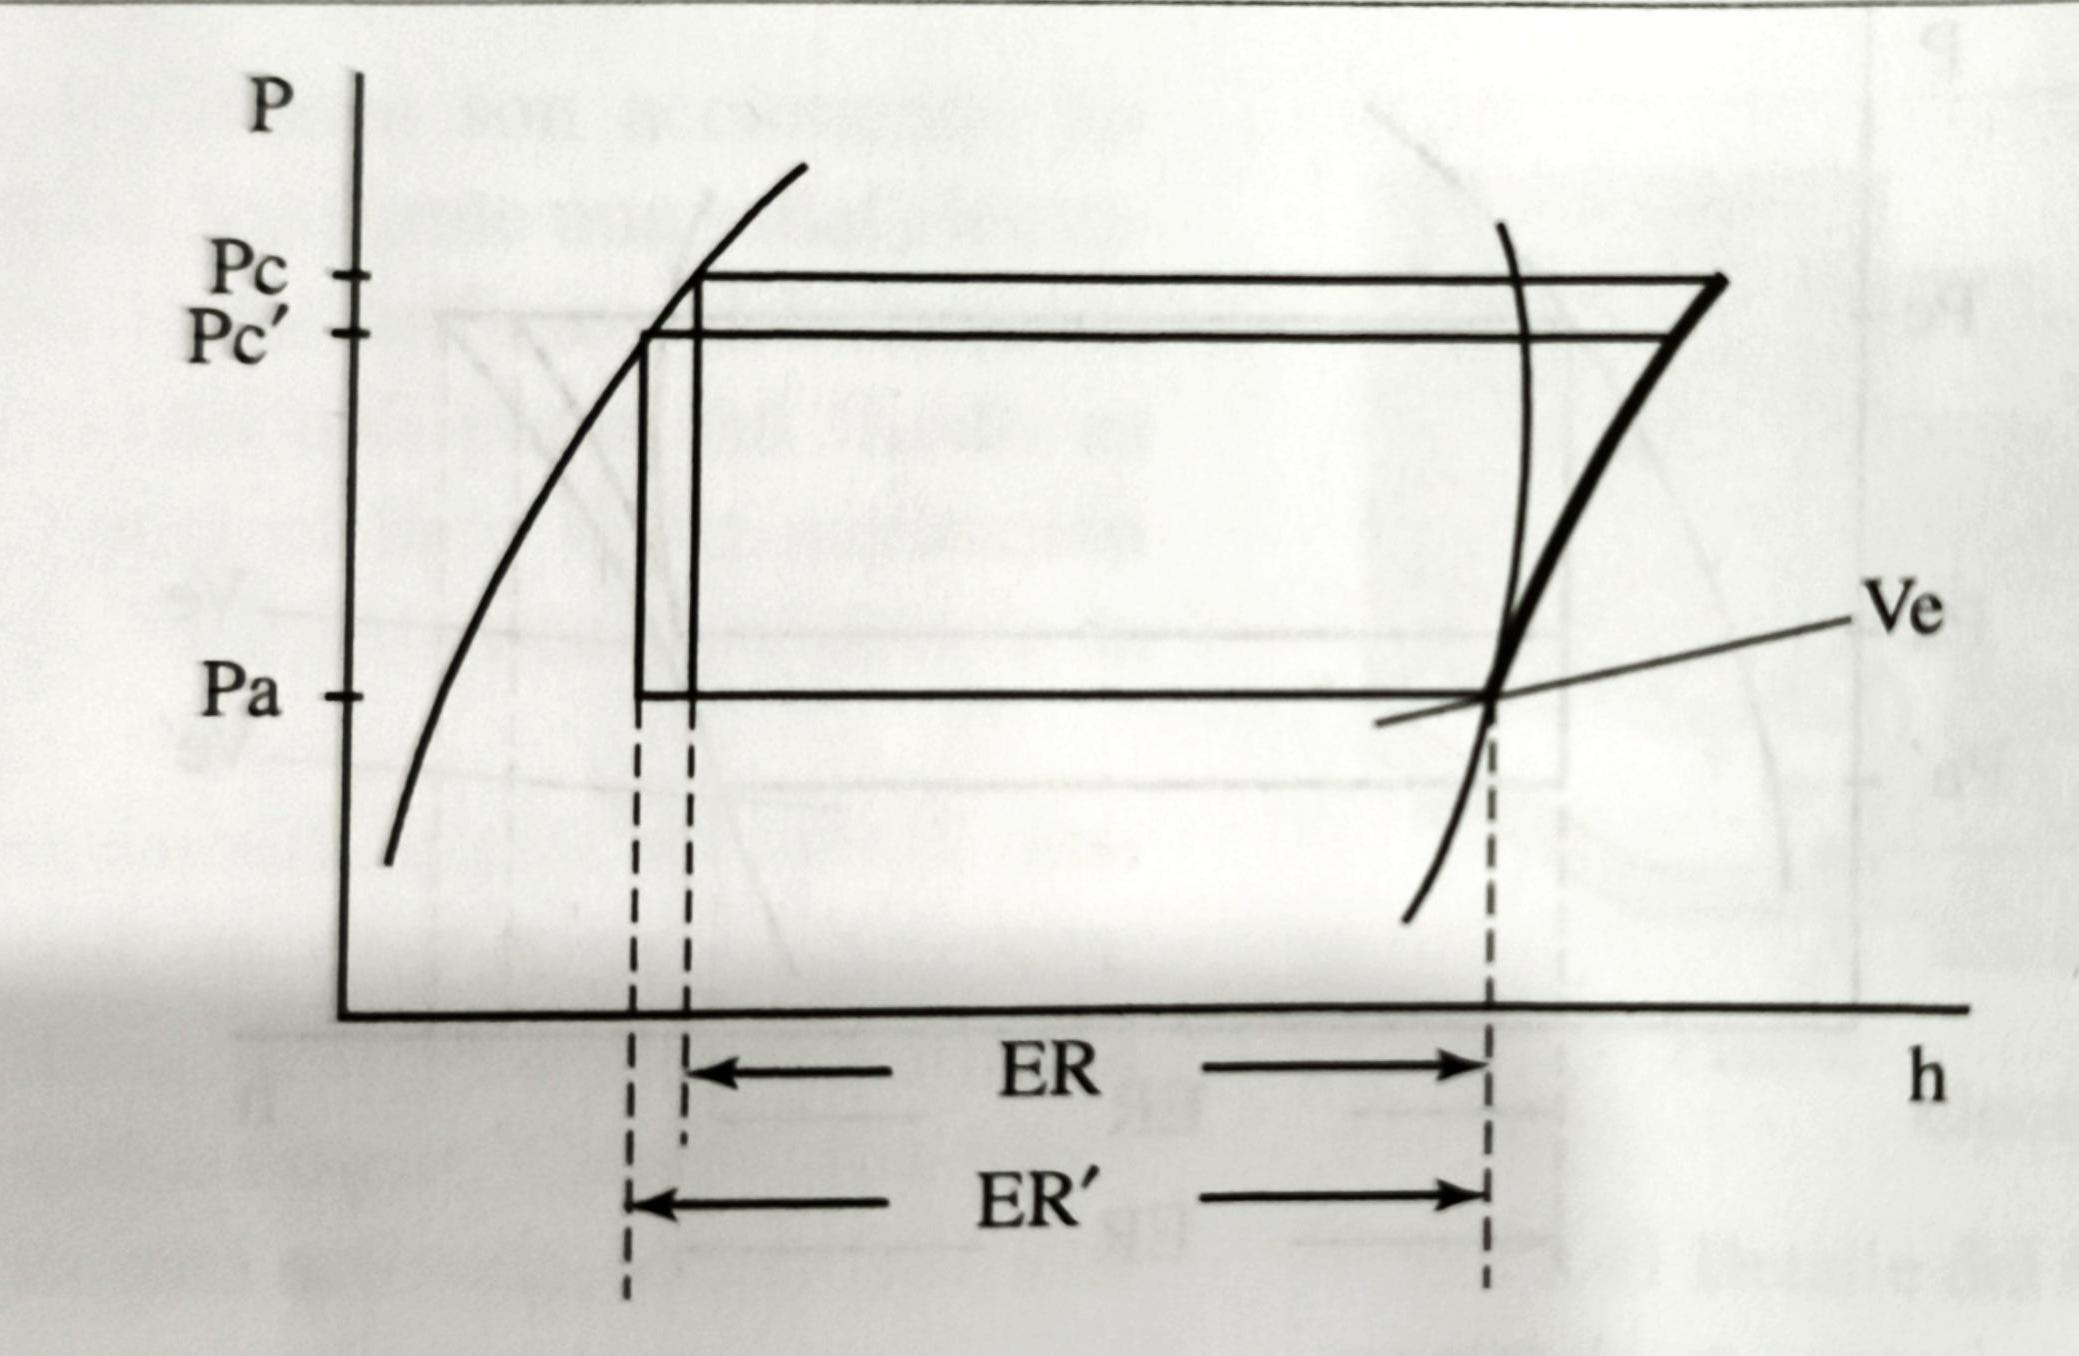
\includegraphics[width=.6\textwidth]{figuras/compresores/variacion de la presion de condensacion.jpg}
		\caption{Variaci\'on de la presi\'on de condensaci\'on en el diagrama p-h}
		\label{fig:Variaci\'on de la presi\'on de condensaci\'on}
	\end{figure}
\end{enumerate}
La \autoref{fig:Capacidad de un compresor modelo 4RD} es un ejemplo es informaci\'on t\'ecnica de un compresor modelo 4RD, en ella podemos corroborar lo anteriormente dicho:
\begin{enumerate}[a.]
	\item Si la temperatura de condensaci\'on es 30\textcelsius\ y de evaporaci\'on -5\textcelsius, entonces su capacidad ser\'a de 11800 kcal/h.
	\item En cambio, si la temperatura de condensaci\'on es de 50\textcelsius\ y la de evaporaci\'on es de -5\textcelsius, entonces su capacidad se reduce a 9400 kcal/h.
\end{enumerate}
\begin{figure}[h]
	\centering
	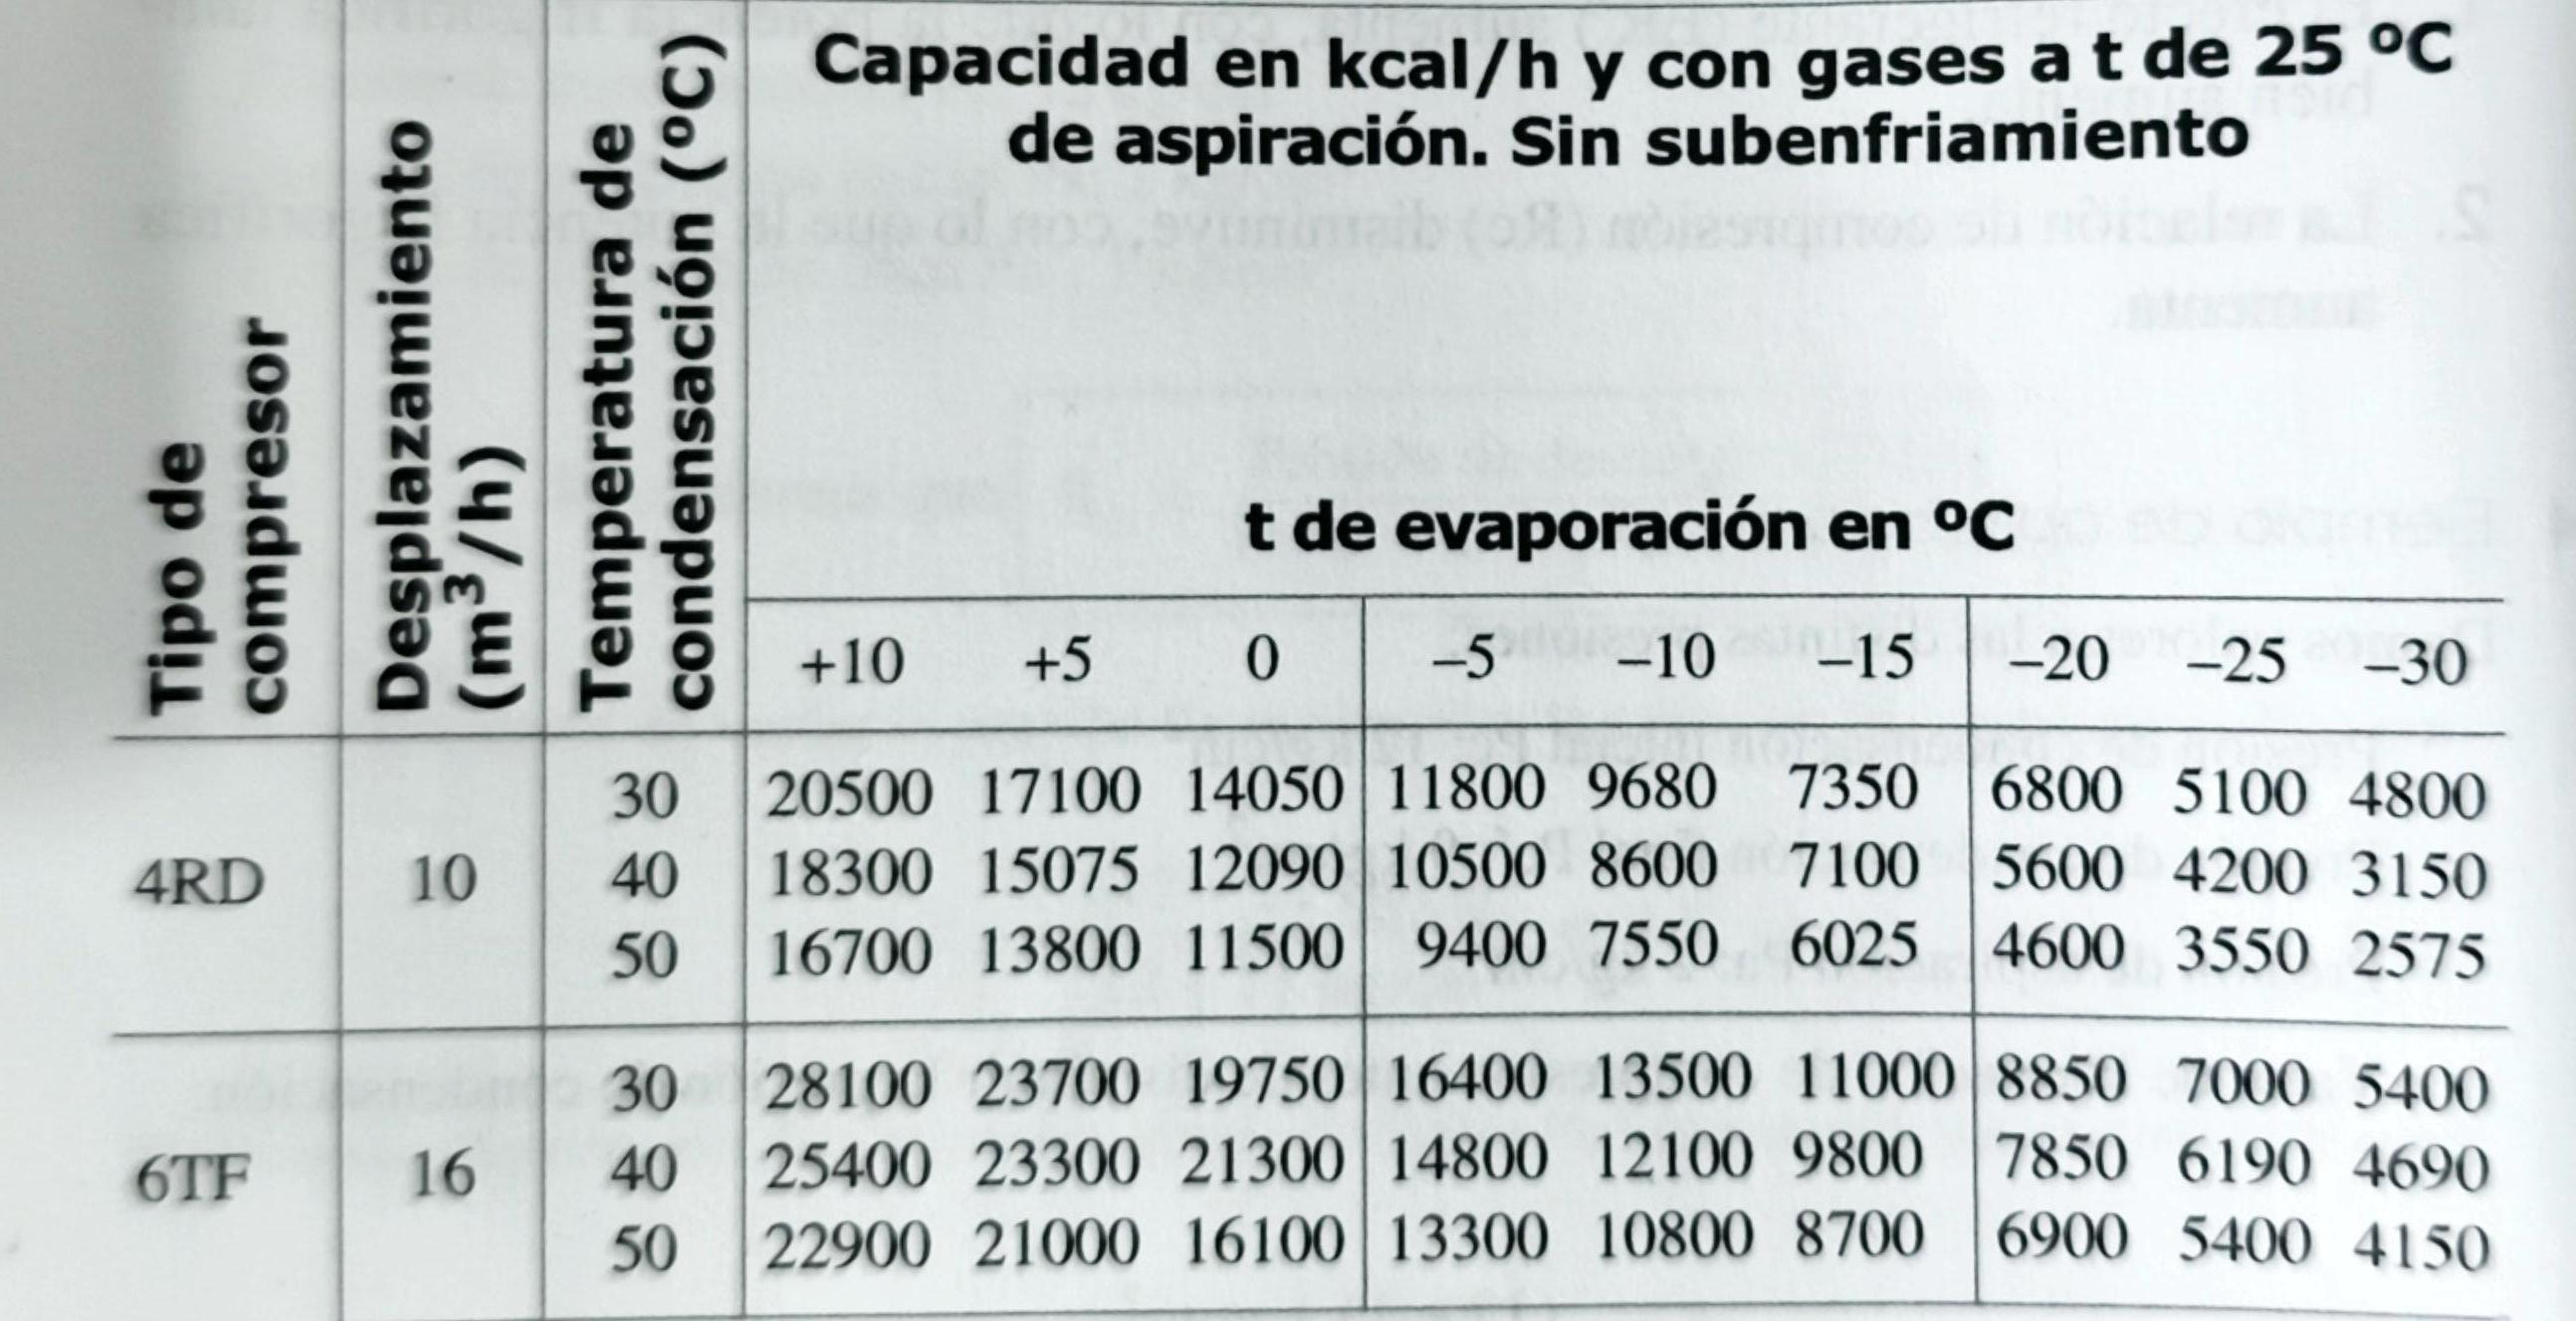
\includegraphics[width=\linewidth]{figuras/compresores/tabla de capacidad de un compresor.jpg}
	\caption{Capacidad de un compresor modelo 4RD}
	\label{fig:Capacidad de un compresor modelo 4RD}
\end{figure}
\subsection{Funcionamiento en régimen seco y en régimen húmedo}
Se dice que trabaja en \textsl{r\'egimen h\'umedo} cuando el fluido a la entrada del compresor es una mezcla de gas y l\'iquido (Tramo 1-2 de la \autoref{fig:R\'egimen seco y h\'umedo}). Esto puede ocurrir por diversas causas, tales como:
\begin{enumerate}[a.]
	\item Mala regulaci\'on del dispositivo de expansi\'on y entra demasiado fluido refrigerante en el evaporador.
	\item Mala circulaci\'on del aire a trav\'es del evaporador por obstrucci\'on o por caudal insuficiente.
\end{enumerate}
Pero en esa mezcla, la cantidad de l\'iquido a\'un no es lo suficiente importante para producir el golpe de l\'iquido, ya que se va evaporando debido a las temperaturas m\'as altas que se va encontrando, por ejemplo:
\begin{enumerate}[a.]
	\item En la conexi\'on tuber\'ia de aspiraci\'on-compresor
	\item En la culata
	\item En el pist\'on
	\item En la camisa
	\item Durante la fase de compresi\'on 
\end{enumerate}

\begin{wrapfigure}{r}{0.5\linewidth}
	\centering
	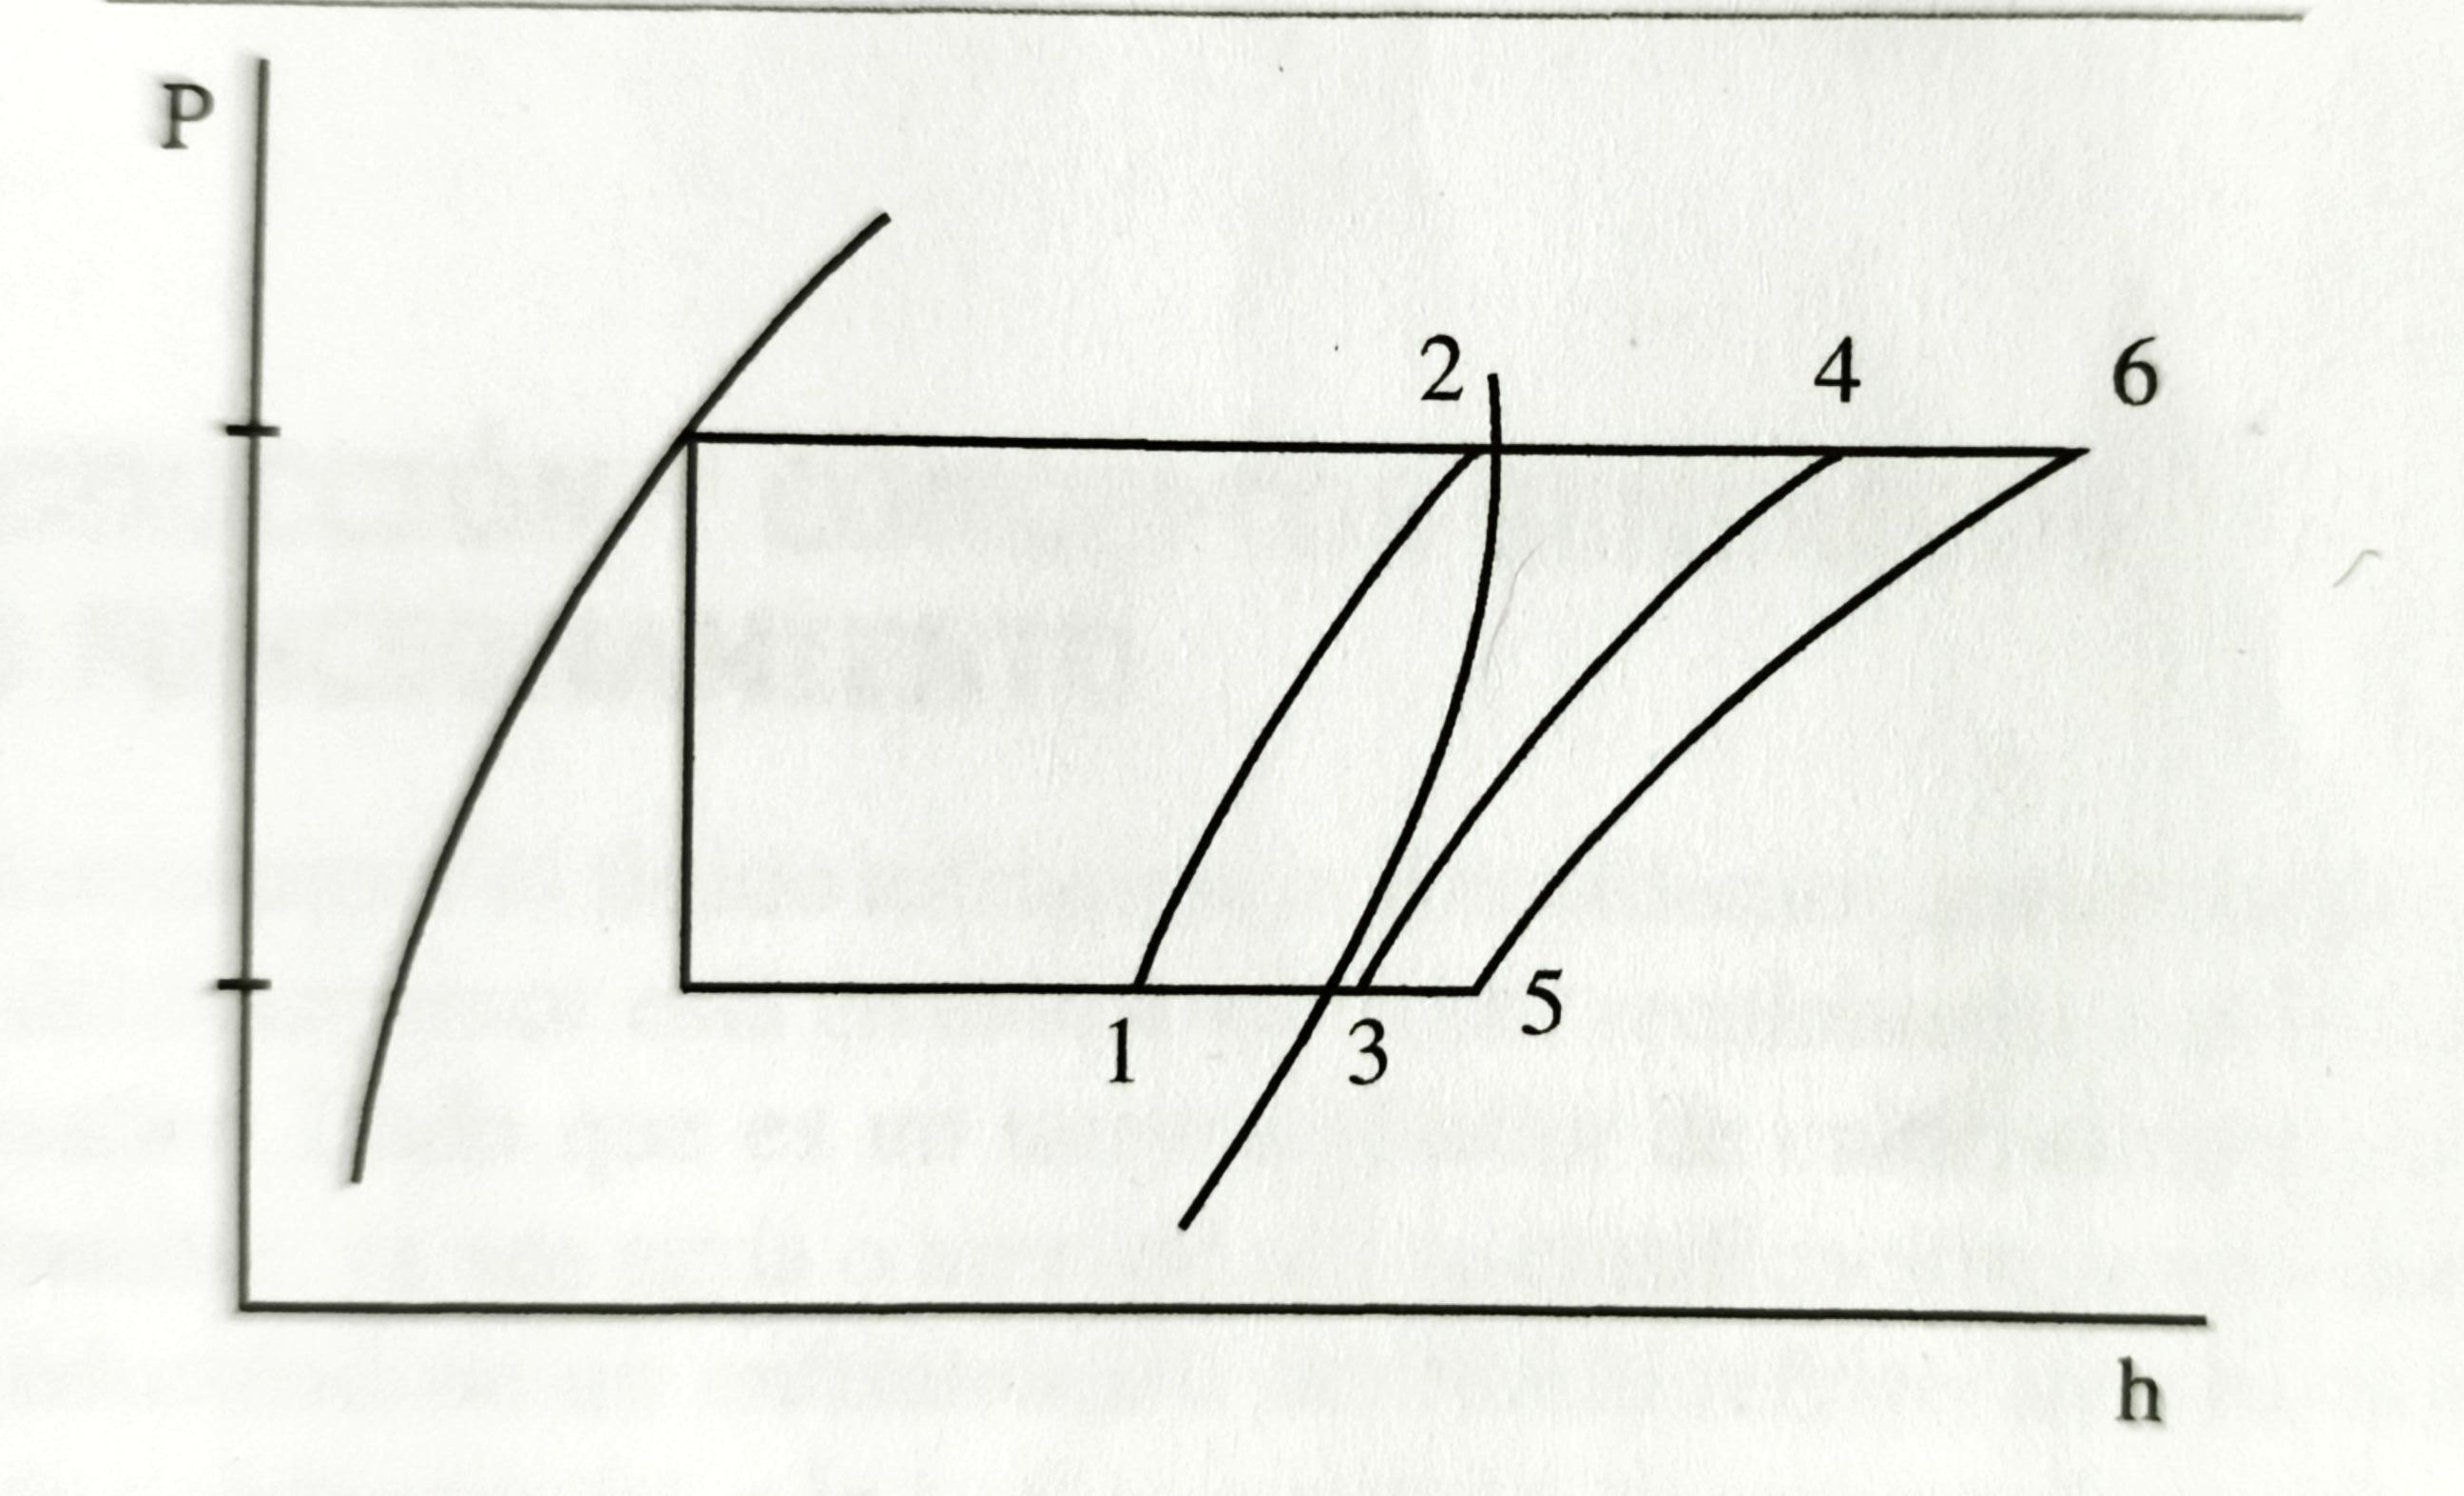
\includegraphics[width=.8\linewidth]{figuras/compresores/régimen seco y humedo.jpg}
	\caption{R\'egimen seco y h\'umedo}
	\label{fig:R\'egimen seco y h\'umedo}
\end{wrapfigure}

Pero ese calor que absorbe el l\'iquido lo est\'a haciendo del calor proveniente del compresor e instalaci\'on y no del ambiente a refrigerar (en el evaporador).\\ En cambio, cuando el fluido a la entrada del compresor es vapor (Tramo 3-4 de la \autoref{fig:R\'egimen seco y h\'umedo}), entonces se trata del \textbf{r\'egimen seco} y, en este caso, el rendimiento es mayor que en el caso anterior. Pero se debe tener especial cuidado para este tipo de funcionamiento, ya que si el vapor que entra al compresor est\'a demasiado sobrecalentado puede generar temperaturas de descarga elevadas por lo que el rendimiento del ciclo ser\'a perjudicado (Tramo 5-6 de la \autoref{fig:R\'egimen seco y h\'umedo}).		